\chapter{Analysis and Results}

\label{chap:results_analyses}

This chapter presents the initial results and analyses from the project, focusing on the setup and validation of the core system components. It covers the datasets utilized for testing the Kafka-ML framework and details the codebase structure for both classic and federated model training architectures.



\section{Dataset}
\label{sec:dataset}

For the initial phase of this project, the primary dataset used for testing and validating the Kafka-ML setup is the \textbf{MNIST dataset}. This widely used dataset of handwritten digits allows for robust testing of the machine learning pipeline, ensuring that the fundamental components for model training and inference are functioning correctly within the Kafka-ML environment.

In the subsequent phases of the project, the focus will shift to integrating and utilizing a \textbf{room occupancy dataset}. This specialized dataset, comprising real-time sensor data (e.g., temperature, humidity, CO2, light levels), will be used to train and evaluate the federated learning model for smart building occupancy prediction, as outlined in the project objectives.



\section{Implementation}
\label{sec:code}

The codebase for this project is managed on GitHub and can be accessed via the following link: \texttt{https://github.com/ertis-research/kafka-ml}. The subsequent sections detail the architecture of the implemented modules.

\subsection{Classic Model Training Architecture}
\label{subsec:classic_model_training}

The classic model training setup within Kafka-ML was configured and tested. This architecture serves as the foundational system before implementing the federated learning components. The key components of this setup include:

\begin{itemize}
    \item \textbf{Frontend:} Provides the user interface or API endpoint for initiating training and inference tasks.
    \item \textbf{Backend:} Manages the machine learning workflows, coordinating the various services.
    \item \textbf{Kafka Control Logger:} Monitors and logs the control messages and status of the different components within the Kafka-ML pipeline.
    \item \textbf{Model Training:} This module handles the actual training of machine learning models. It supports:
    \begin{itemize}
        \item TensorFlow
        \item PyTorch
    \end{itemize}
    \item \textbf{Model Inference:} This module is responsible for making predictions using the trained models. It supports:
    \begin{itemize}
        \item TensorFlow
        \item PyTorch
    \end{itemize}
\end{itemize}

\subsection{Federated Learning Module Architecture}
\label{subsec:federated_learning_module}

Federated deployments reuse the classic Kafka-ML services (frontend, backend API, model training, model inference) and add asynchronous coordination so that models and client datasets remain decoupled until a federated round is ready. Figure~\ref{fig:fed_arch_flow} (to be added) will illustrate the flow; the key stages are summarised below.

\begin{enumerate}
    \item \textbf{User orchestration via Frontend/Backend:} Operators configure models and deployments through the standard frontend. The backend persists those definitions and emits control messages, extending the classic workflow with federated-specific metadata.

    \item \textbf{Federated model initialisation (`model\_training/tensorflow`):} When a federated deployment starts, the TensorFlow job assigns a unique federated identifier, creates per-round Kafka topics, publishes a ``federated model logger'' message, pushes the serialised model to the model data topic, and advertises its location via the model control topic.

    \item \textbf{Model control path:} The Federated Model Control Logger consumes the logger event, validates it, and forwards the control envelope to the Federated Backend, which caches the global model metadata while it waits for the matching data control signal.

    \item \textbf{Data control path:} Edge devices or simulators publish metadata to the federated data control topic. The Federated Data Control Logger consumes and normalises these records before relaying them to the Federated Backend. Each control payload identifies the Kafka topic that stores the actual training samples.

    \item \textbf{Triggering a training round:} Once the backend has both model and data control messages for the same identifier, it launches the Kubernetes job defined in `federated\_model\_training/tensorflow`, providing the cached envelopes so the job can read the referenced topics.

    \item \textbf{Client-side training on federated workers:} Each federated worker downloads the advertised model artefact, ingests the Kafka topic holding its data shard, and performs local optimisation (optionally honouring streaming-chunk schedules or dynamic sampling weights). After training the worker publishes both performance metrics and the new weight payload to the aggregation topics so the coordinator can retrieve them.

    \item \textbf{Aggregation and global model refresh:} The aggregation service consumes the worker submissions, validates the accompanying control messages, applies the configured aggregation rule (FedAvg in the current deployment), and writes the updated global weights back to Kafka. Metrics are streamed to the backend so dashboards reflect round progress, and the final model is promoted through the existing inference path to keep downstream behaviour aligned with the classic deployment.
\end{enumerate}

These stages deliver a repeatable pipeline: the classic services continue to manage user workflows, while the additional loggers, backend hooks, and Kubernetes jobs orchestrate federated training across Kafka topics dedicated to model artefacts, control signals, and data streams.

\subsection{Federated Learning with Blockchain Integration}
\label{subsec:federated_blockchain}

When blockchain support is enabled, the same federated orchestration pipeline gains an immutable audit trail and automated incentives. The control/data choreography remains unchanged, but additional steps bind every critical message to a smart contract and wallet maintained for that deployment.

\begin{enumerate}
    \item \textbf{Backend wallet initialisation:} During deployment the backend provisions (or links) a dedicated wallet that tracks balance and outbound rewards for the federated job. The wallet address and contract identifiers are stored alongside the model configuration so every component can reference them.

    \item \textbf{Control message notarisation:} After the model training service emits the federated model control message to Kafka, it also writes the same payload (hash plus metadata) to the blockchain contract. This establishes a tamper-evident record that downstream consumers can verify before accepting the round.

    \item \textbf{On-chain logging of client updates:} Each federated worker, once local training finishes, pushes its contribution metadata to the blockchain contract in parallel with the aggregation control topic. The contract stores the association between client wallet, round identifier, and performance metrics.

    \item \textbf{Aggregated model attestation:} The aggregation service consumes the client control messages as usual, fetches the updated weights, and publishes the new global model. In addition, it records the aggregation outcome on-chain (including the Kafka topic that holds the refreshed weights) so the blockchain ledger mirrors the state of the global model.

    \item \textbf{Reward calculation and settlement:} Using the metrics submitted by the workers, the aggregation service (or a dedicated reward handler) computes contribution deltas against the previous round—considering loss reduction, accuracy gains, and other configured KPIs. The resulting token or credit transfer is executed via the federated deployment’s wallet, issuing payments to client accounts and logging the transaction hash back into the backend for reporting.
\end{enumerate}

This extension preserves the privacy benefits of Kafka-ML’s federated mode while adding non-repudiation, transparent contribution history, and automated incentive distribution managed through the blockchain contract.

\section{KafkaML Setup}


\subsection{Setup and Execution of Classic Model Training with MNIST}
\label{subsec:classic_mnist_setup}

This section outlines the steps undertaken to set up and validate the classic model training architecture within Kafka-ML using the MNIST dataset as shown in Fig. \ref{fig:collage1}. The process involved containerizing the application, deploying it to a local Kubernetes cluster, and subsequently utilizing the Kafka-ML frontend to perform model training and inference.

\paragraph{Dockerization and Kubernetes Deployment}
The initial phase involved preparing the Kafka-ML codebase for containerized deployment. This included:
\begin{itemize}
    \item Building the necessary Docker images for the various components of the classic architecture (Frontend, Backend, Model Training, Model Inference). This step also involved adopting the required dependencies and making necessary code adjustments to ensure compatibility and smooth execution within a containerized environment.
    \item Pushing the built Docker images to a Docker registry, making them accessible for deployment.
    \item Developing Kustomization scripts to manage the configuration of the Kafka-ML application for deployment on a Kubernetes cluster.
    \item Deploying the Kafka-ML application to a local Minikube cluster, simulating a cloud-native environment on the local machine.
\end{itemize}


\begin{figure}[h!]
    \centering
    \begin{adjustbox}{bgcolor=gray!20, padding=0.7em, margin=1ex}
        \begin{tabular}{cc}
            \begin{subfigure}{0.48\textwidth}
                \centering
                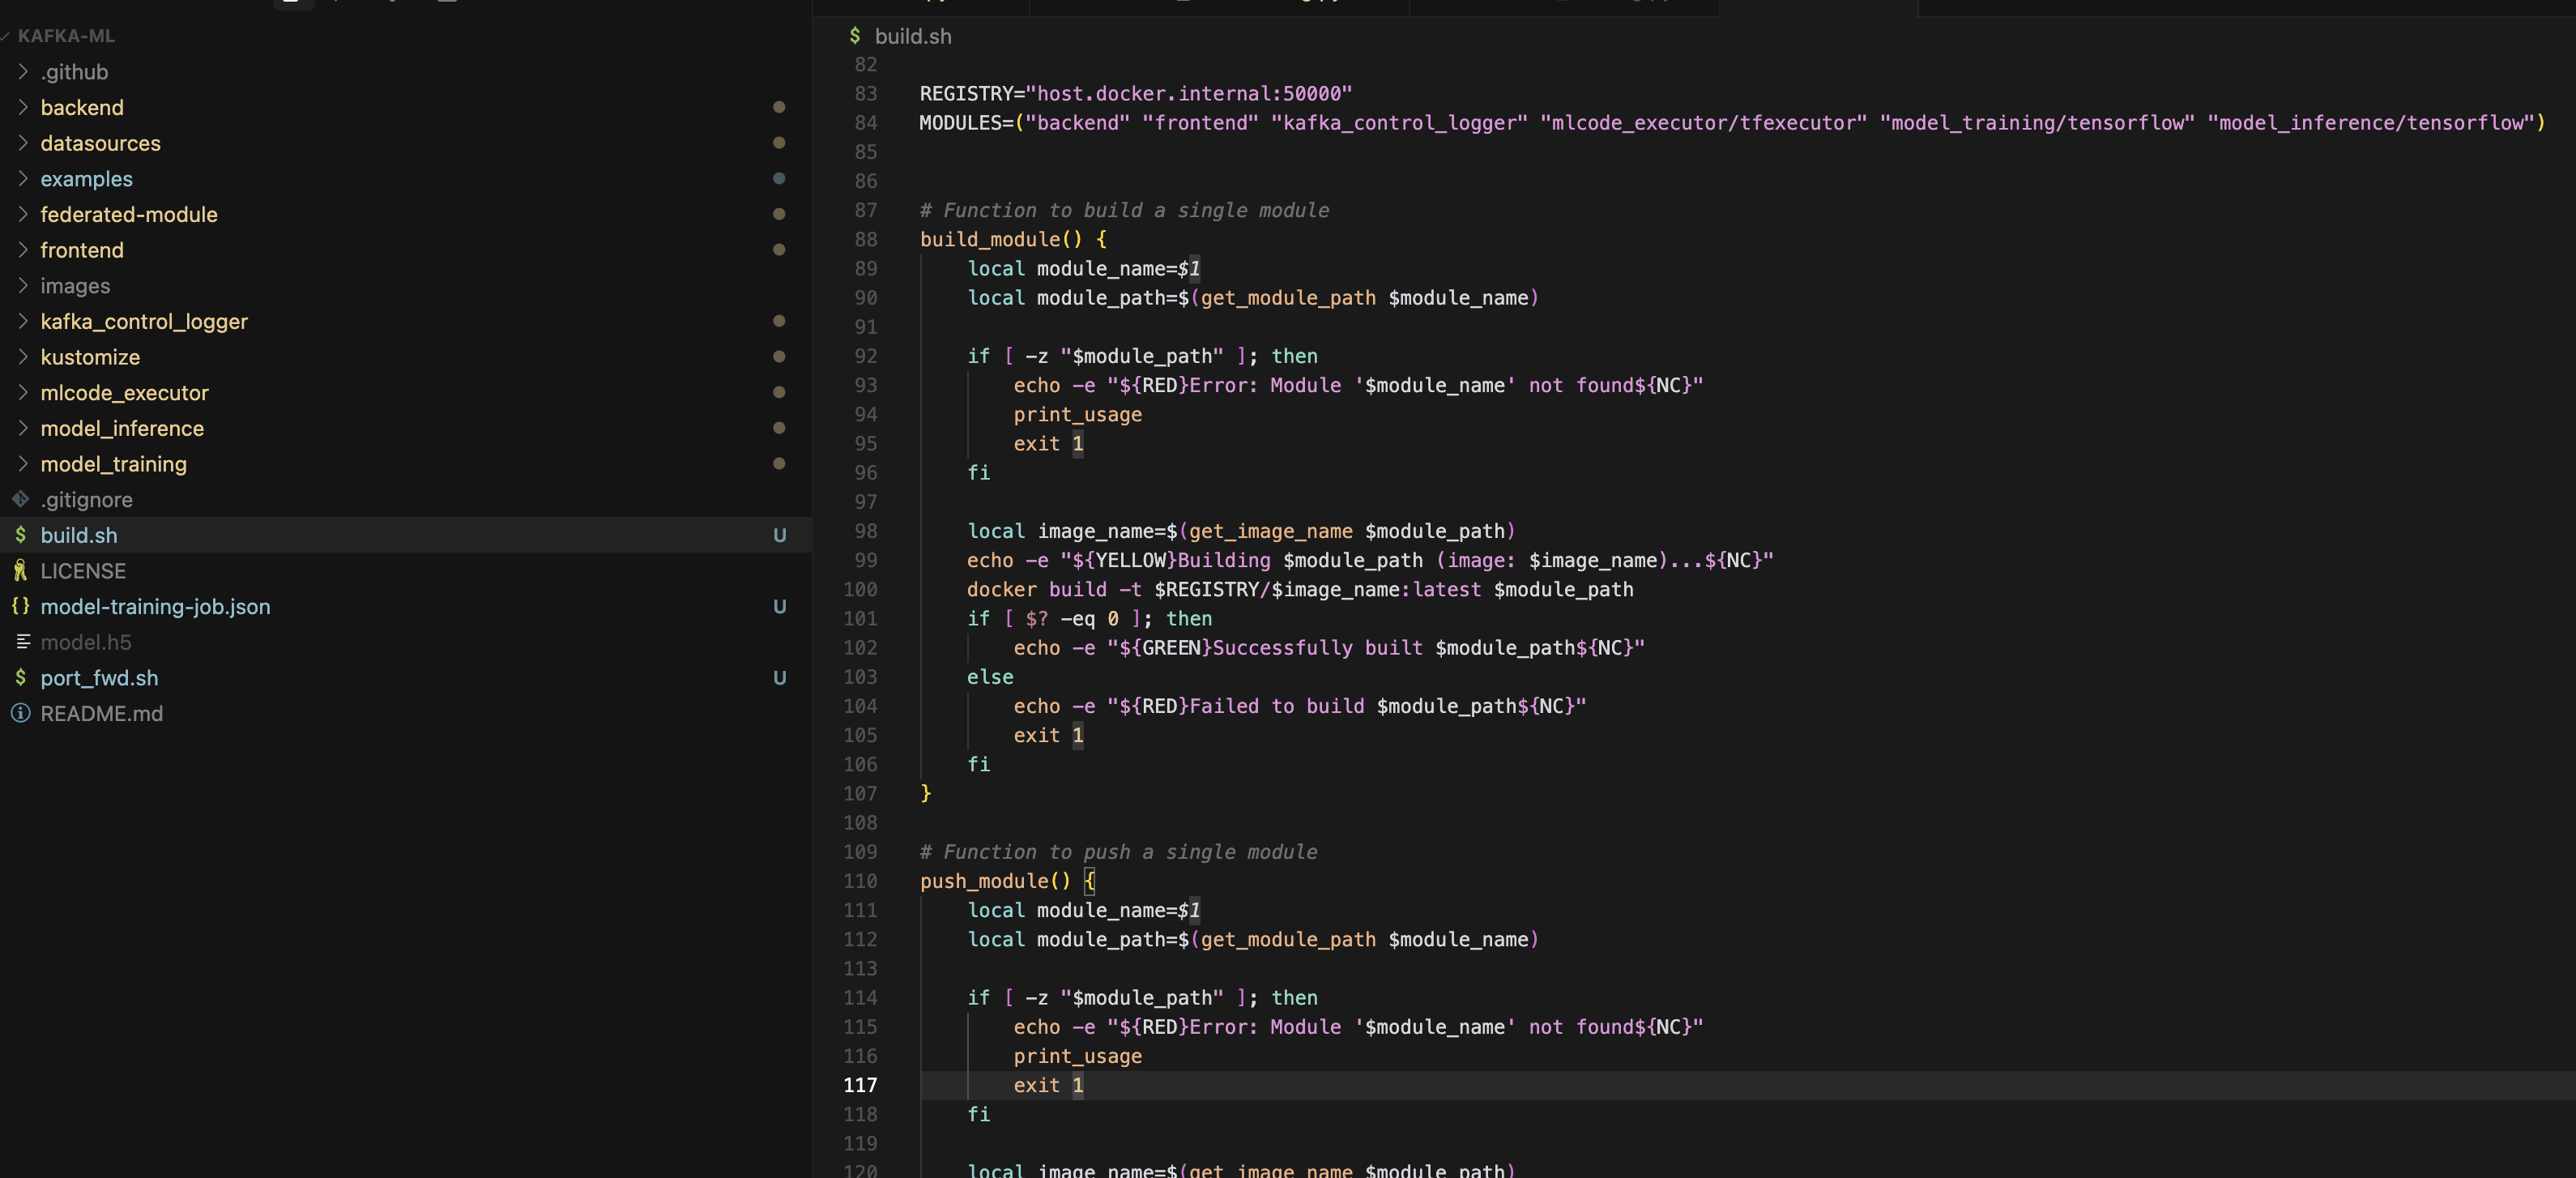
\includegraphics[width=\linewidth]{MWP-Project Report Template - BD-ML-June25/screenshots_classic/1_build_script.png}
                \caption{Build Script}
            \end{subfigure} &
            \begin{subfigure}{0.48\textwidth}
                \centering
                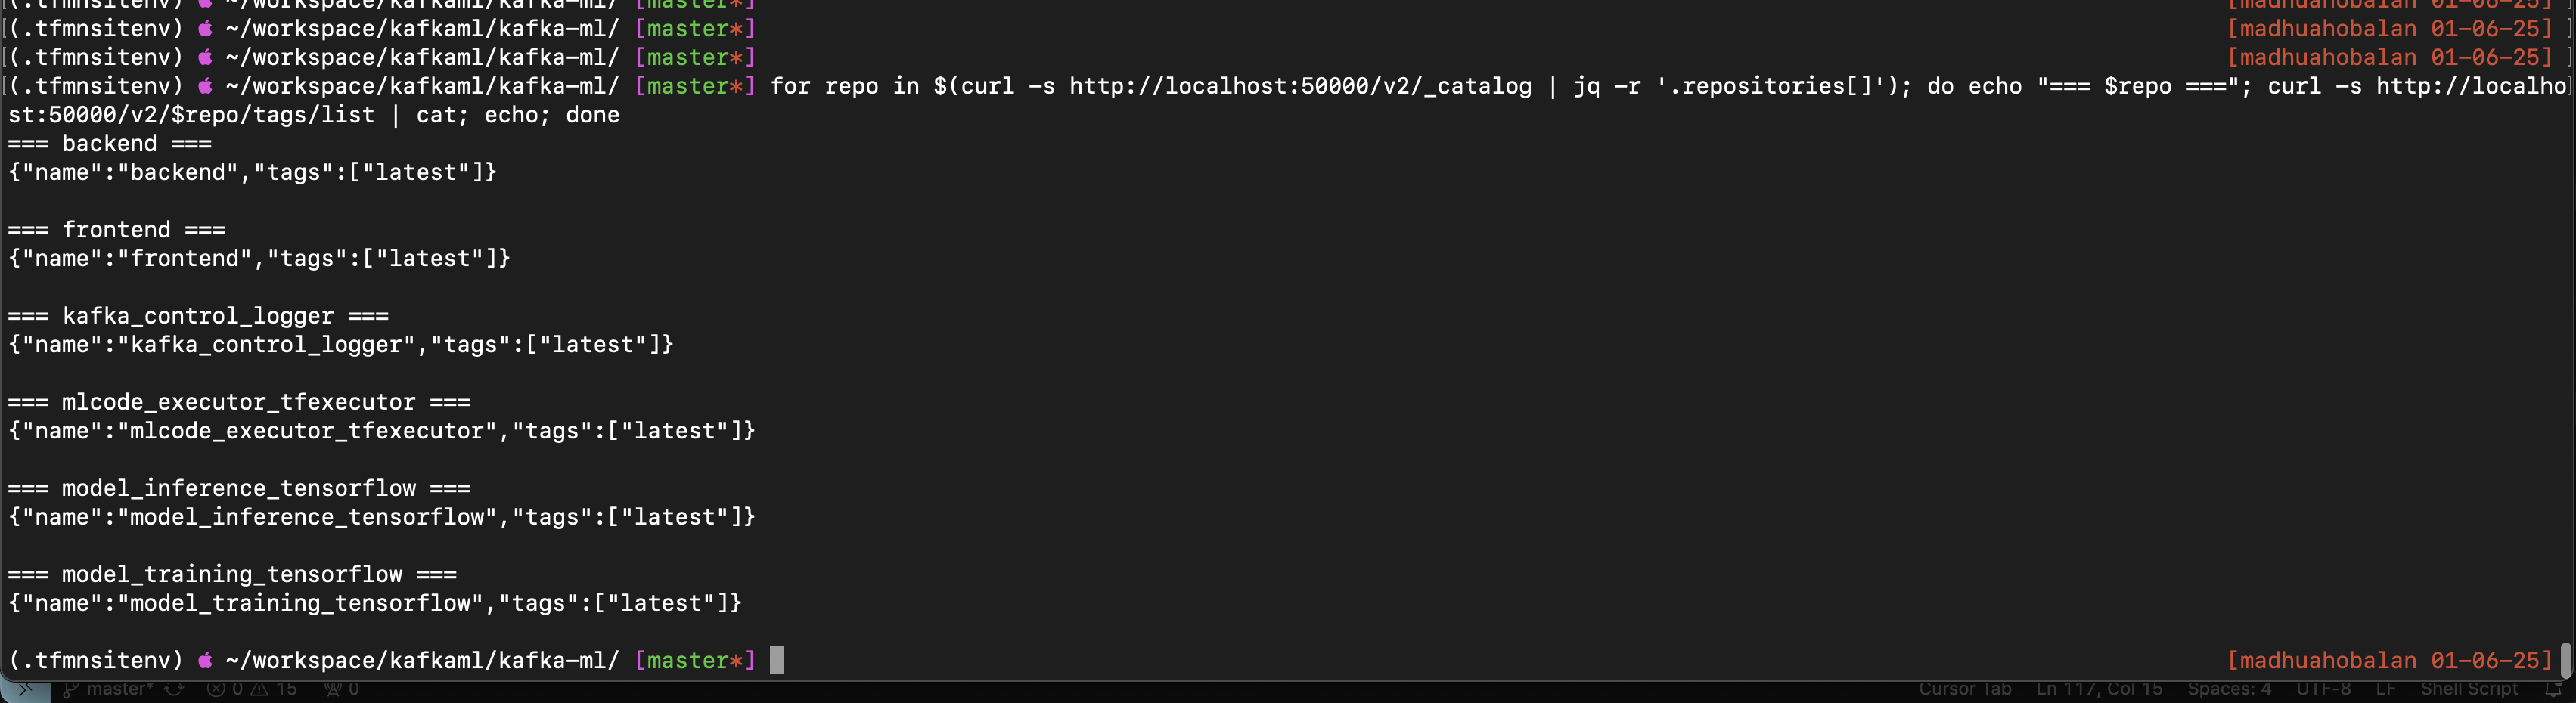
\includegraphics[width=\linewidth]{MWP-Project Report Template - BD-ML-June25/screenshots_classic/2_local_docker_registry.png}
                \caption{Docker Images}
            \end{subfigure} \\
            % Second row
            \begin{subfigure}{0.48\textwidth}
                \centering
                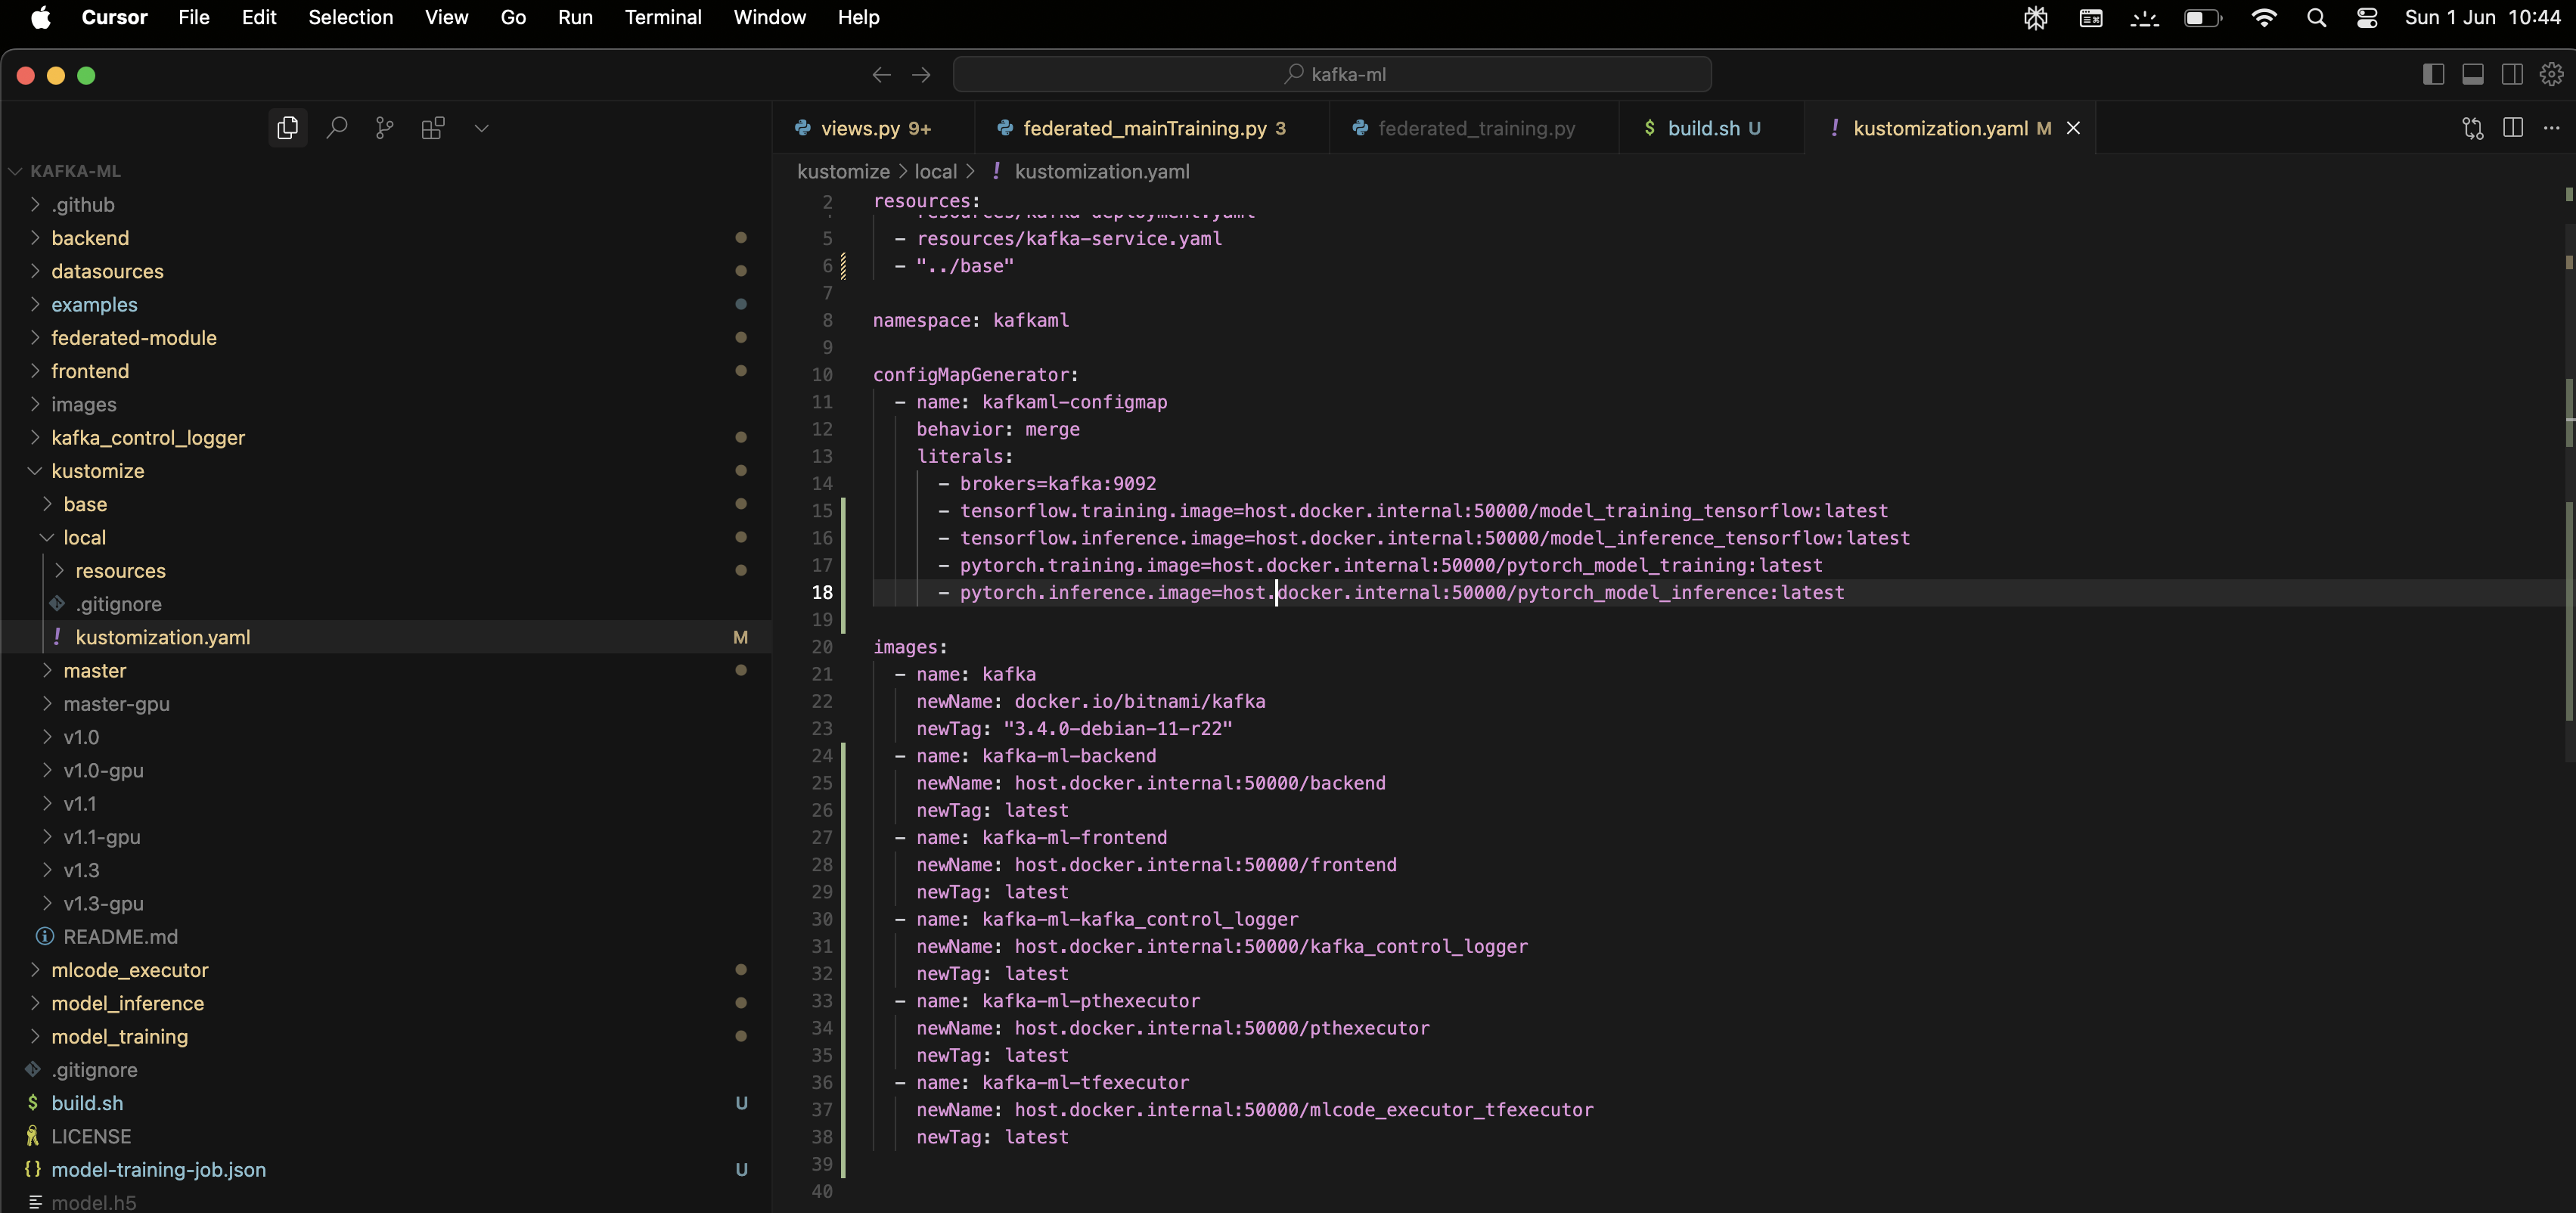
\includegraphics[width=\linewidth]{MWP-Project Report Template - BD-ML-June25/screenshots_classic/3_kustomise_depliyment_script.png}
                \caption{Deployment Script}
            \end{subfigure} &
            \begin{subfigure}{0.48\textwidth}
                \centering
                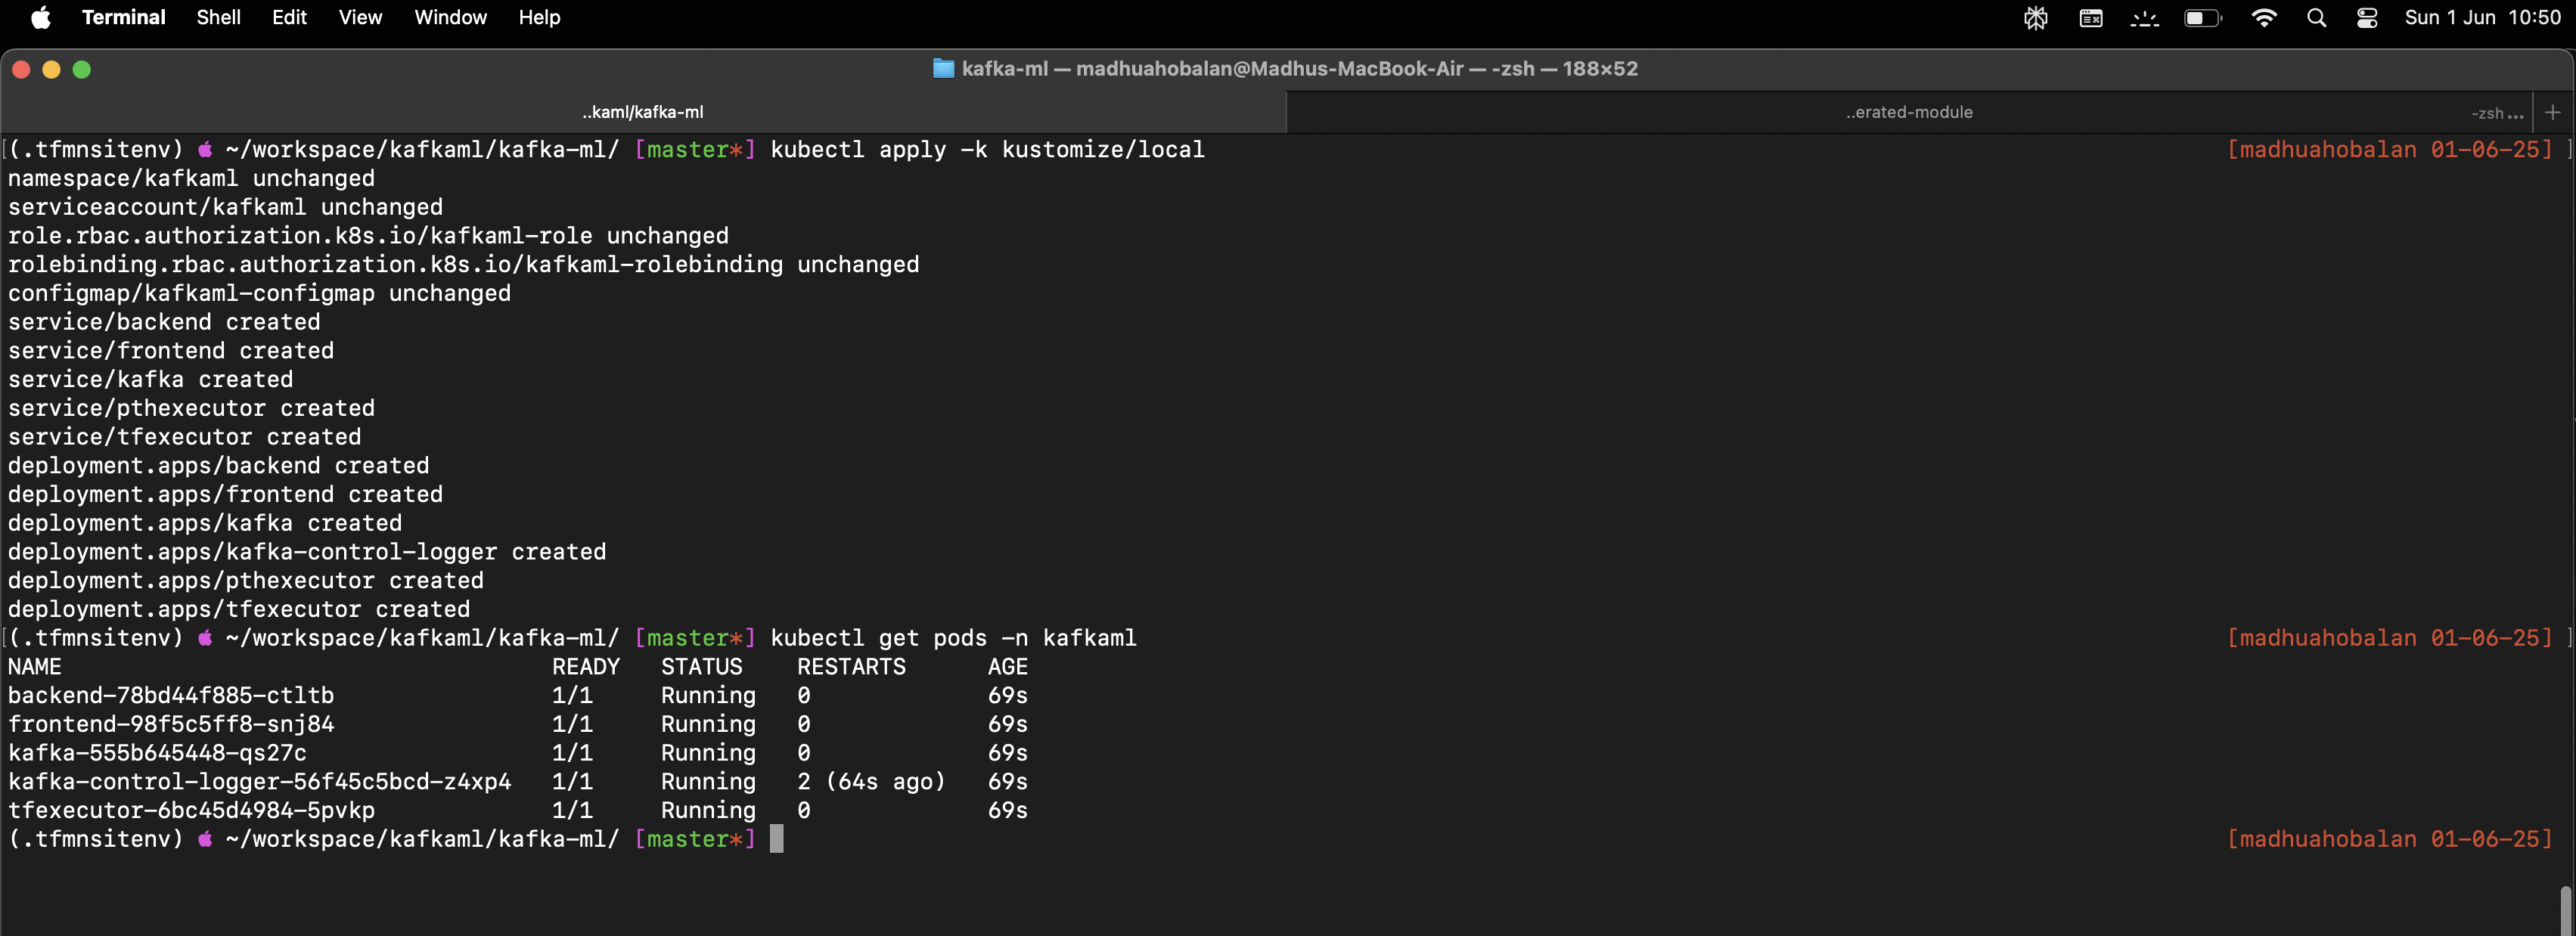
\includegraphics[width=\linewidth]{MWP-Project Report Template - BD-ML-June25/screenshots_classic/4_running_local_pods.png}
                \caption{Running Kubernetes Pods}
            \end{subfigure}
        \end{tabular}
    \end{adjustbox}
    \vskip\baselineskip
    \caption{Kafka ML Build and Deploy Steps}
    \label{fig:collage1}
\end{figure}


\paragraph{Model Training and Inference via Kafka-ML Frontend}
Once the Kafka-ML system was successfully deployed on Minikube, the frontend application was accessed via a web browser to perform the end-to-end machine learning workflow:

\begin{enumerate}
    \item \textbf{Adding a TensorFlow Model:} A TensorFlow model suitable for the MNIST dataset was added to the Kafka-ML system through its frontend interface as depicted in Fig. \ref{fig:collage-model1}.
    % Placeholder for a screenshot of adding a model
\begin{figure}[h!]
    \centering
    \begin{adjustbox}{bgcolor=gray!20, padding=0.7em, margin=1ex}
        \begin{subfigure}{0.5\textwidth}
            \centering
            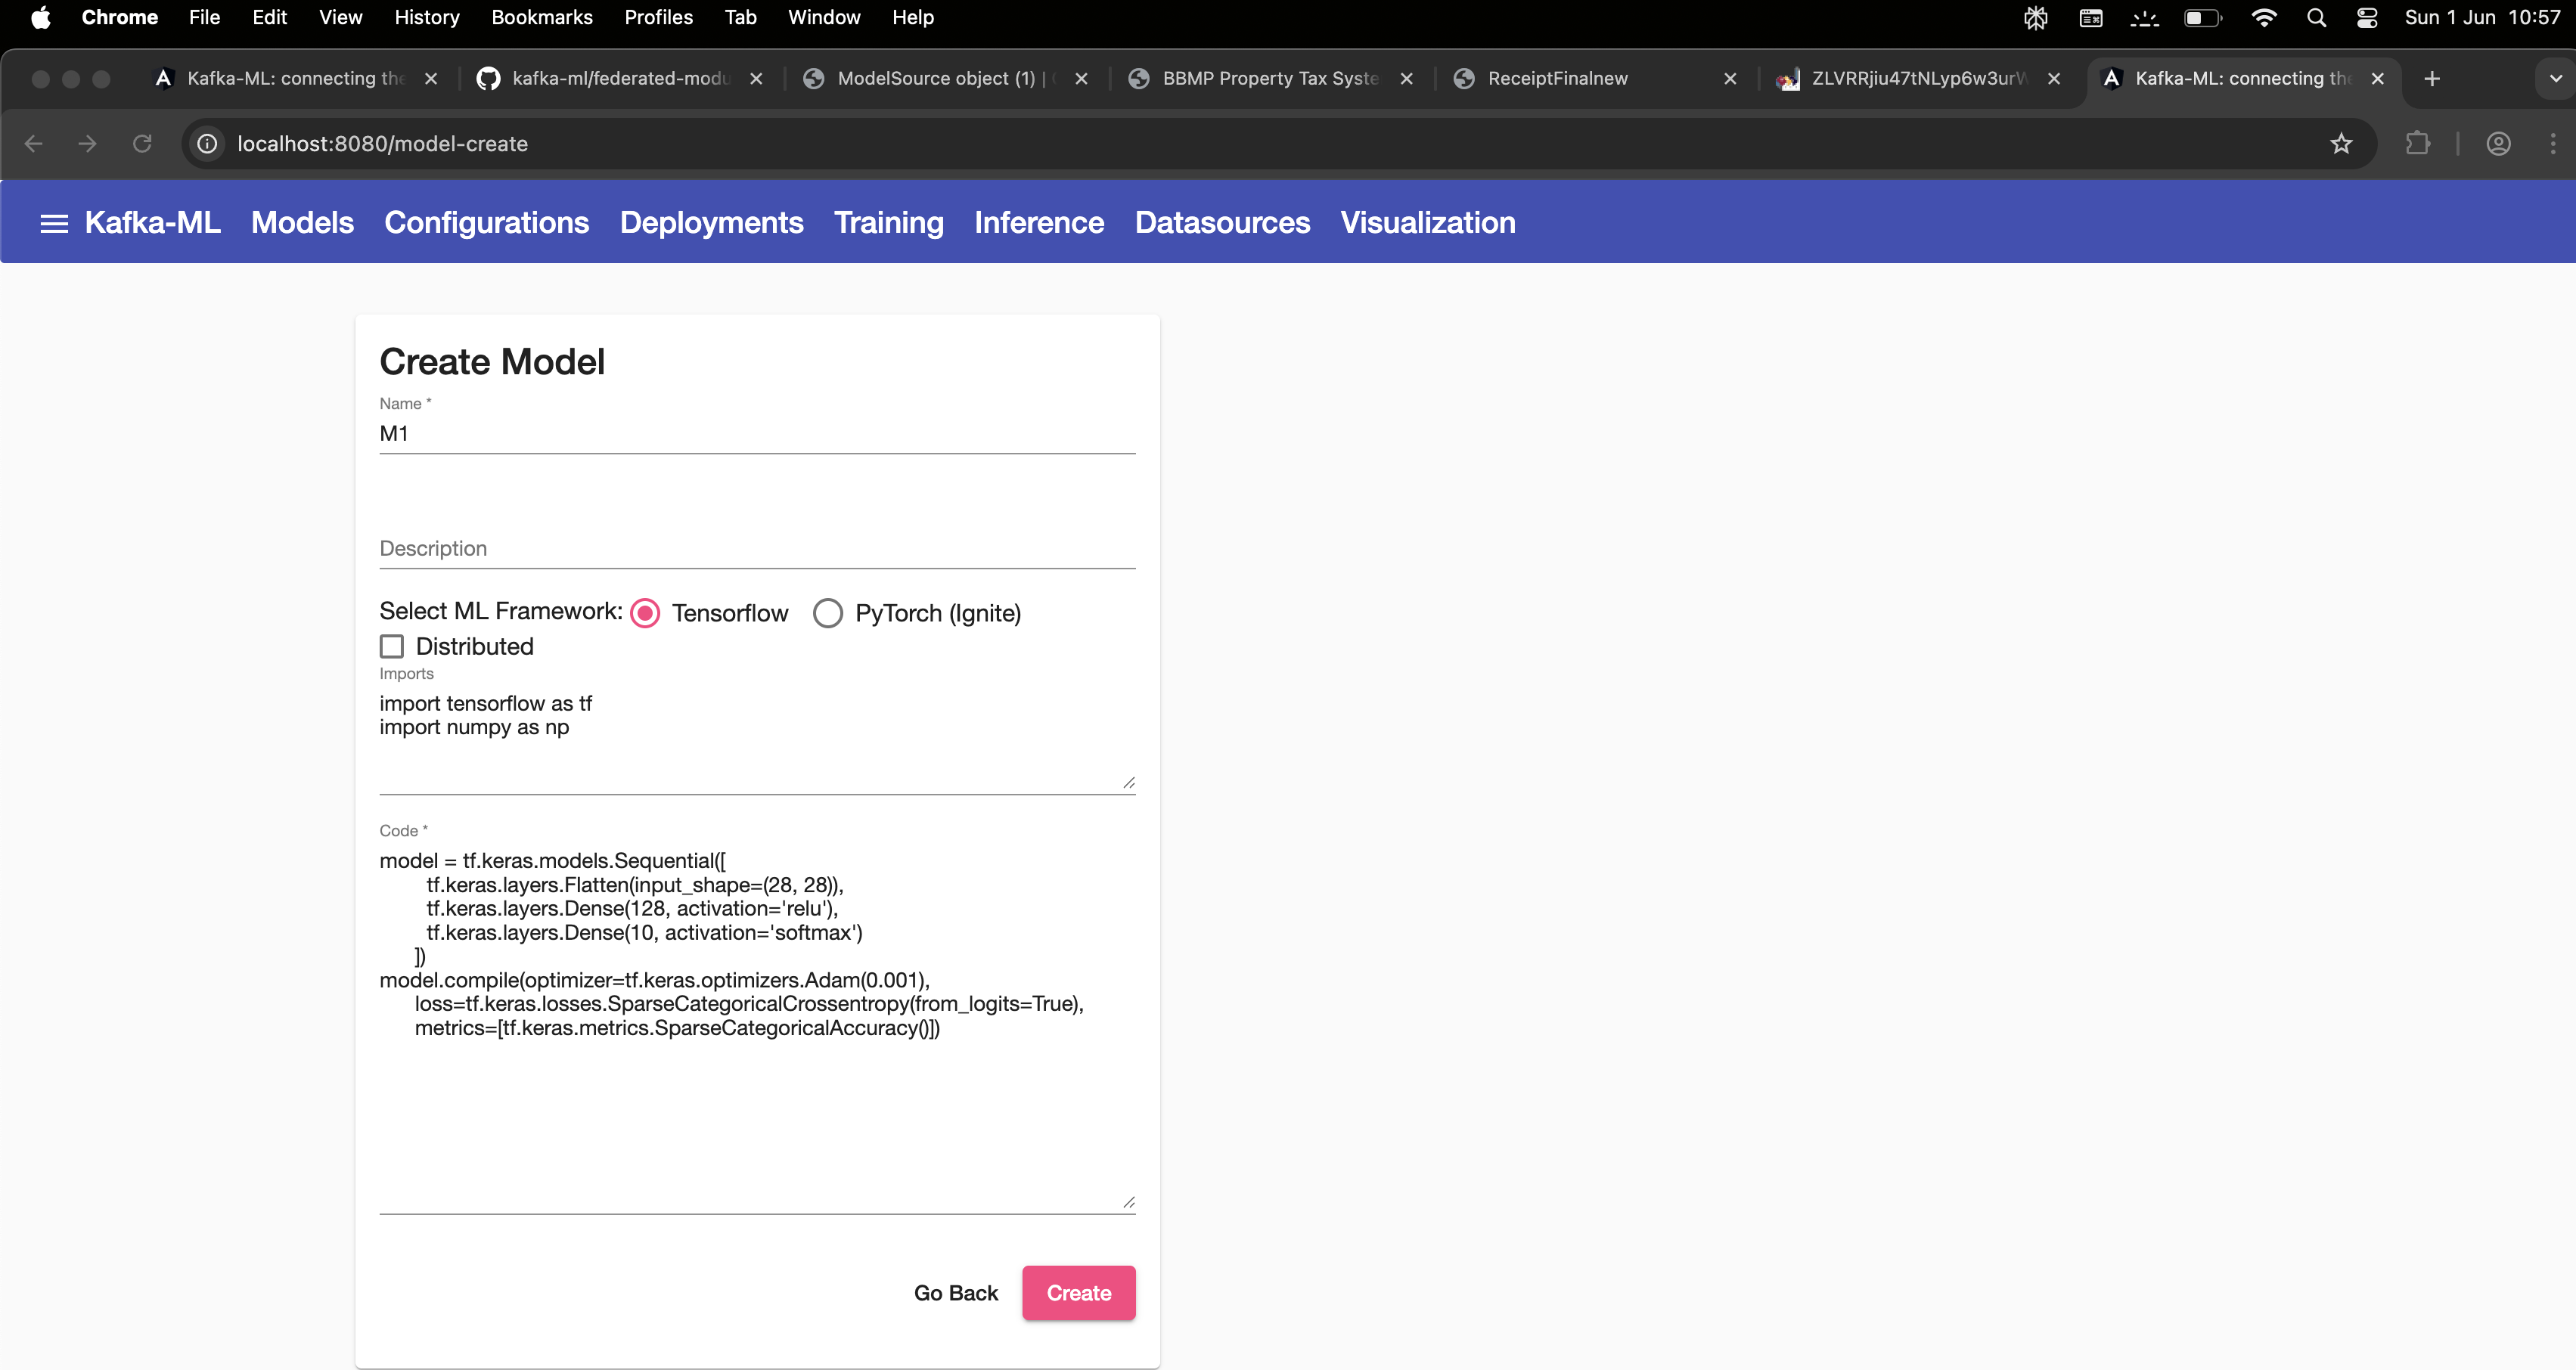
\includegraphics[width=\linewidth]{MWP-Project Report Template - BD-ML-June25/screenshots_classic/5_Model_Creation.png}
            \caption{Model Inputs}
        \end{subfigure}
        \hfill
        \begin{subfigure}{0.5\textwidth}
            \centering
            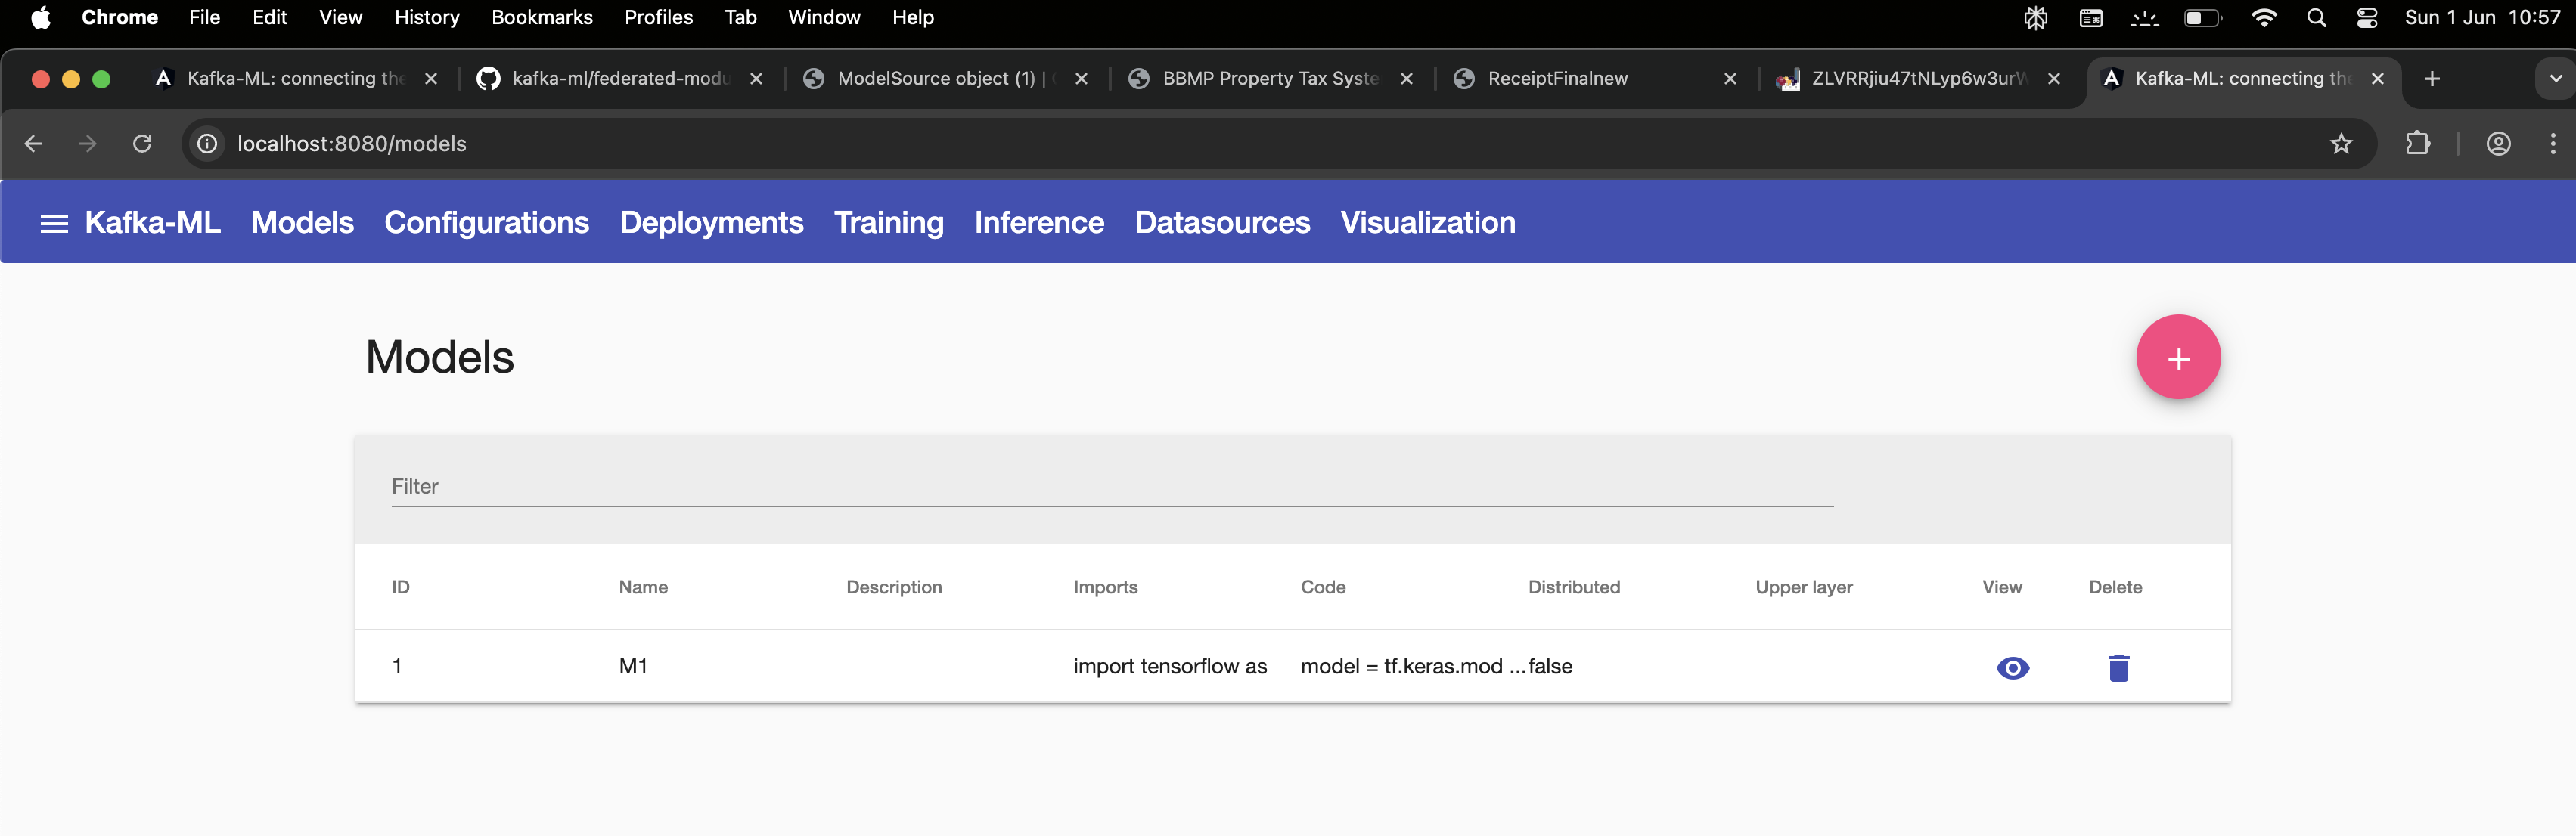
\includegraphics[width=\linewidth]{MWP-Project Report Template - BD-ML-June25/screenshots_classic/5a_model_created.png}
            \caption{Created Model}
        \end{subfigure}
    \end{adjustbox}
    \vskip\baselineskip
    \caption{Adding a TensorFlow model for MNIST classification}
    \label{fig:collage-model1}
\end{figure}

    \item \textbf{Creating Model Configuration:} A configuration was created for the added TensorFlow model, specifying parameters such as training settings, dataset details (MNIST), and other relevant hyperparameters and sample screnshots are given in Fig. \ref{fig:collage-config2}.
    % Placeholder for a screenshot of model configuration

\begin{figure}[h!]
    \centering
    \begin{adjustbox}{bgcolor=gray!20, padding=0.7em, margin=1ex}
        \begin{subfigure}{0.5\textwidth}
            \centering
            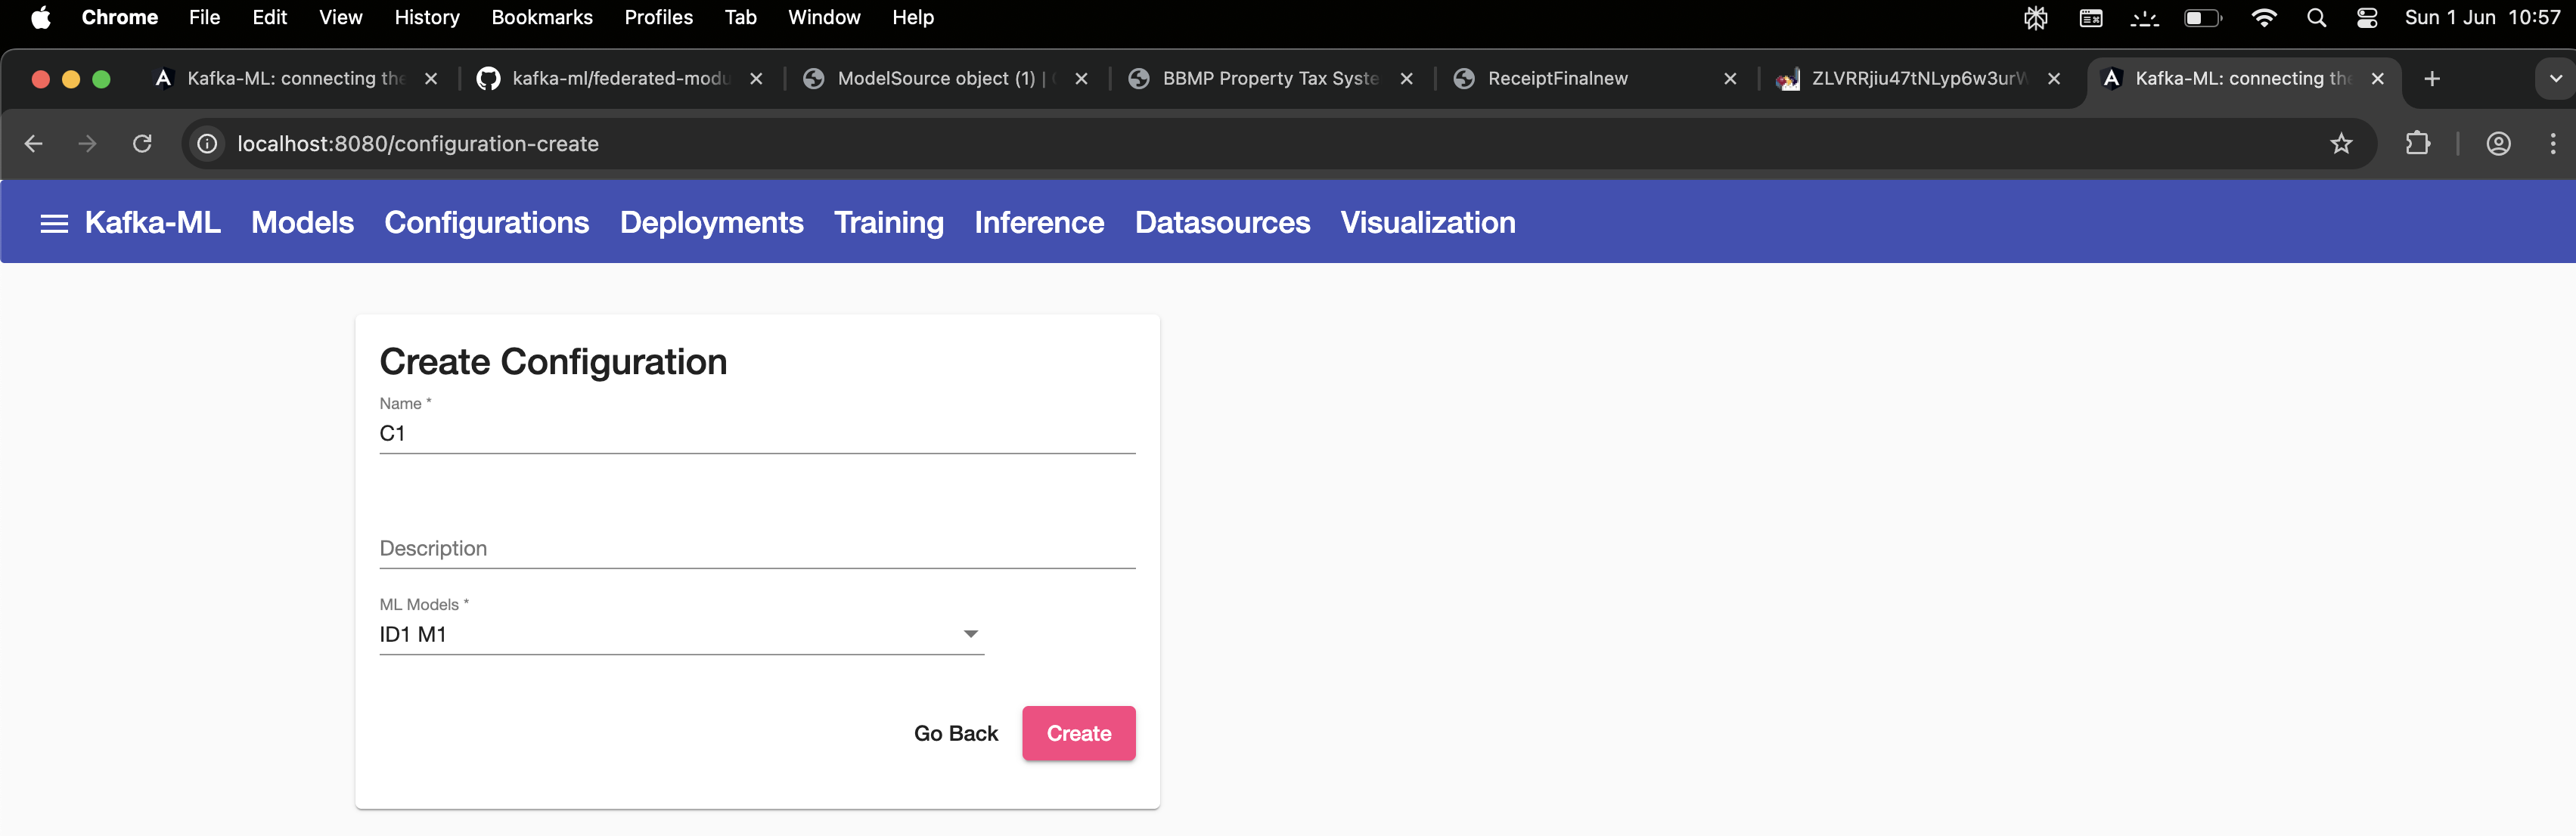
\includegraphics[width=\linewidth]{MWP-Project Report Template - BD-ML-June25/screenshots_classic/6_Config_Creation.png}
            \caption{Configuration Inputs}
        \end{subfigure}
        \hfill
        \begin{subfigure}{0.5\textwidth}
            \centering
            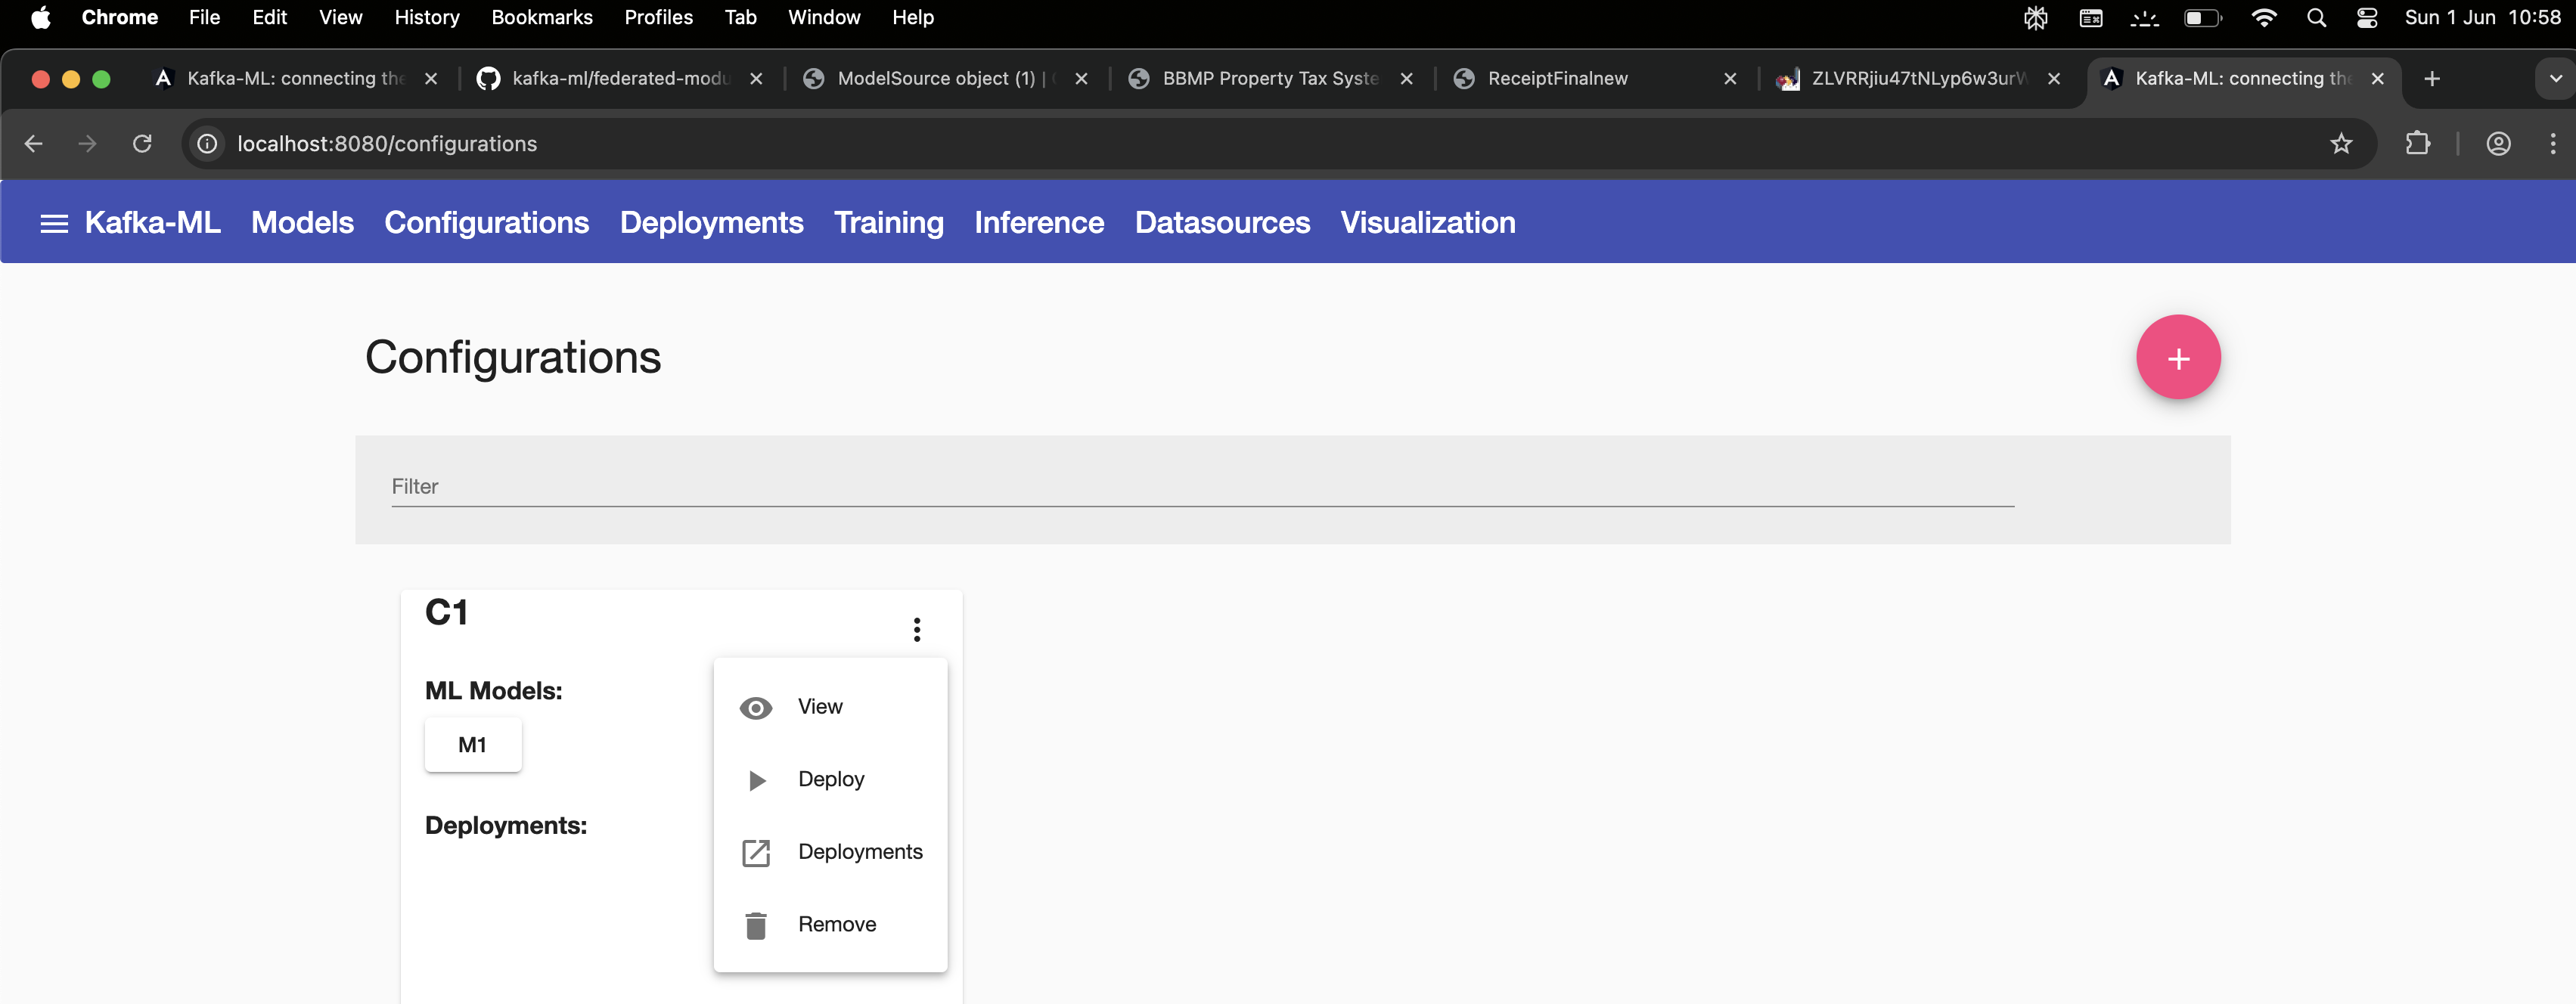
\includegraphics[width=\linewidth]{MWP-Project Report Template - BD-ML-June25/screenshots_classic/6a_configuration_created.png}
            \caption{Created Configuration}
        \end{subfigure}
    \end{adjustbox}
    \vskip\baselineskip
    \caption{Configuration setup for the MNIST TensorFlow model.}
    \label{fig:collage-config2}
\end{figure}

    \item \textbf{Creating a Deployment:} Based on the model and its configuration, a deployment was created within Kafka-ML as shown in Fig. \ref{fig:collage3}. This makes the model available for training and subsequent inference tasks.

\begin{figure}[h!]
    \centering
    \begin{adjustbox}{bgcolor=gray!20, padding=0.7em, margin=1ex}
        \begin{tabular}{cc}
            % First row
            \begin{subfigure}{0.5\textwidth}
                \centering
                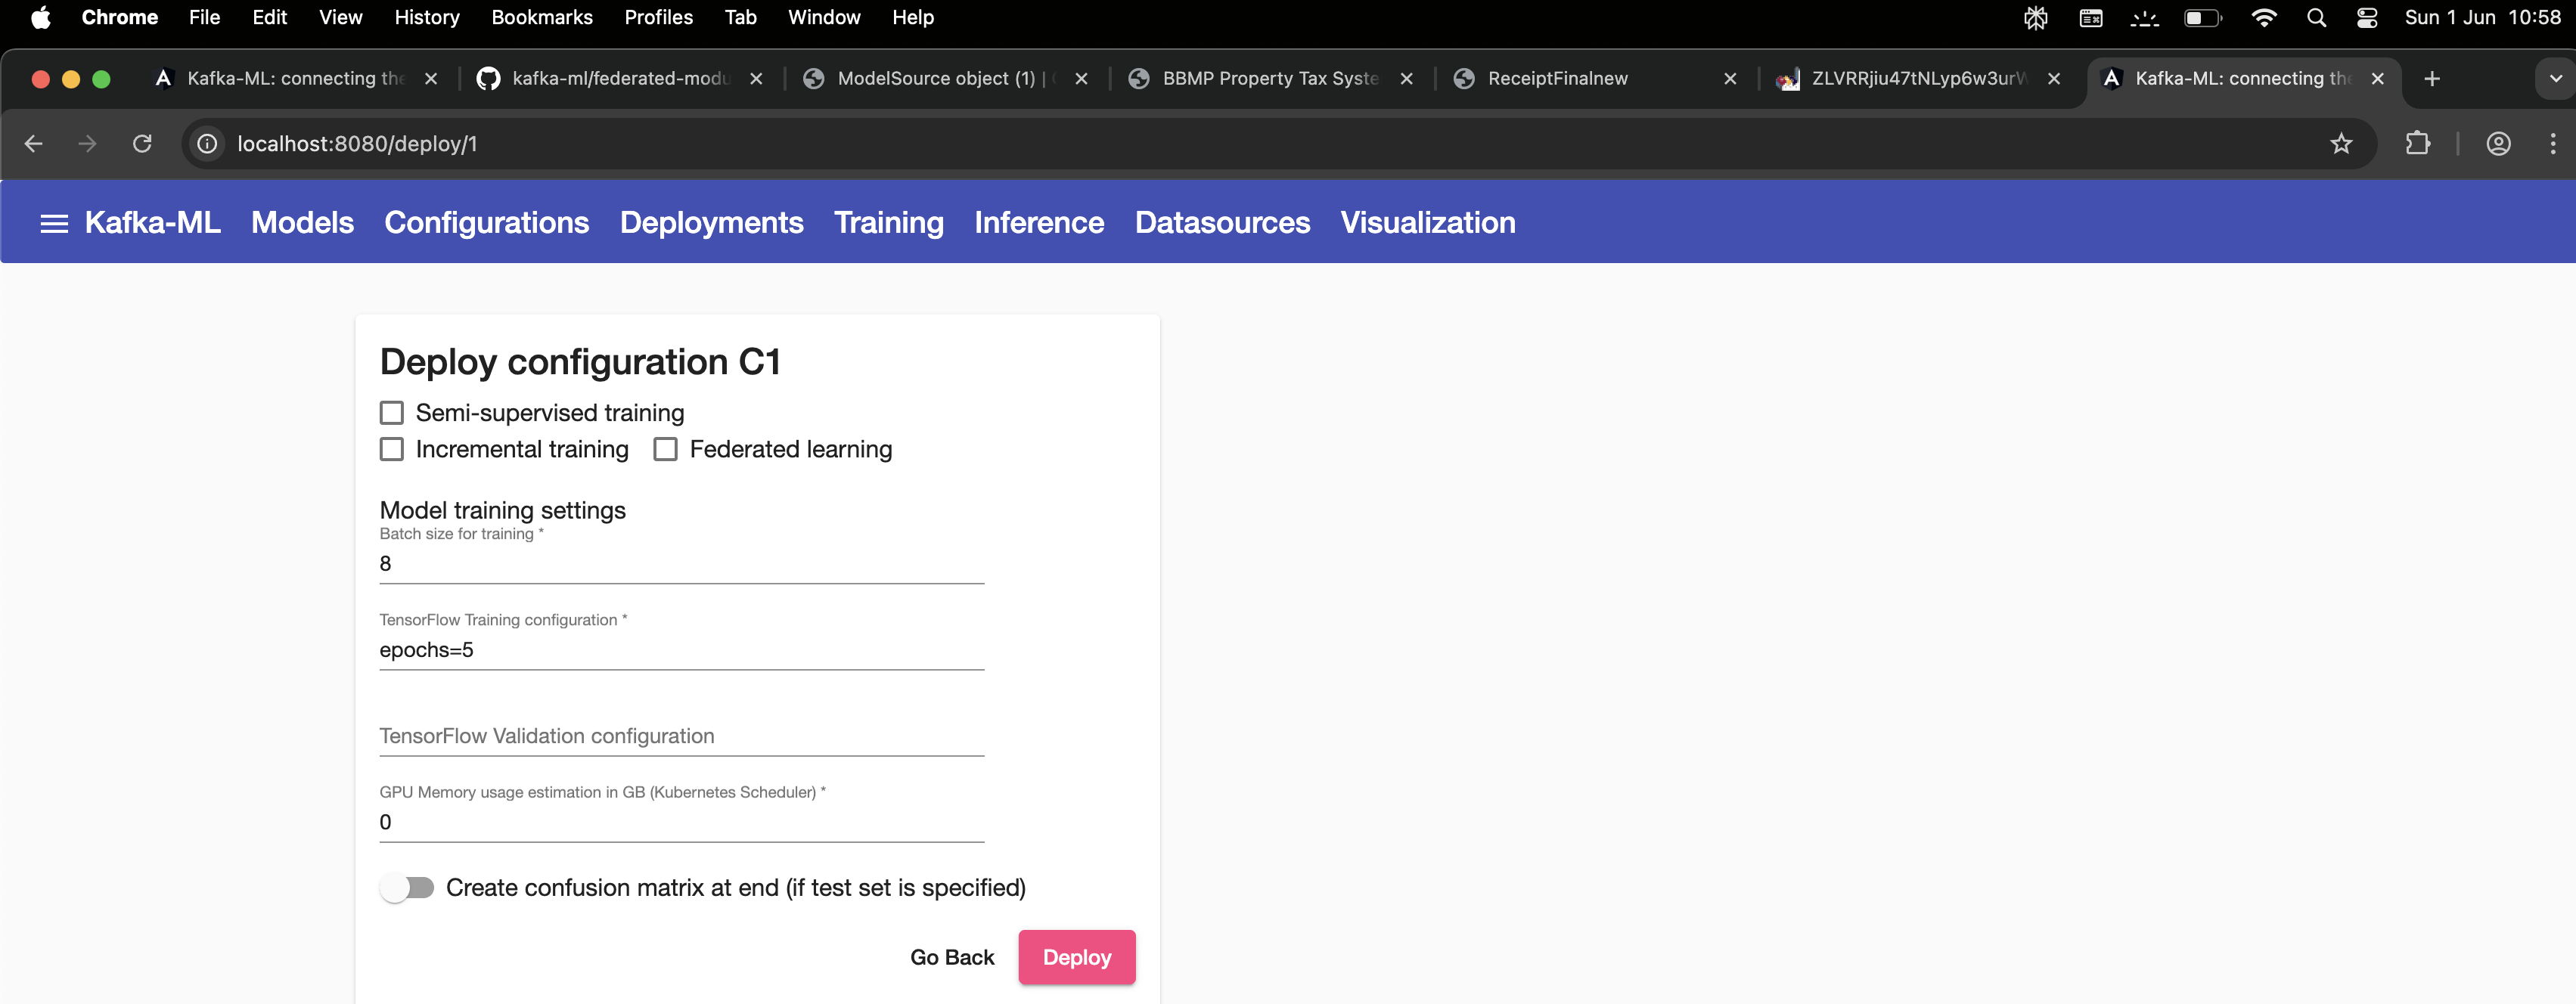
\includegraphics[width=\linewidth]{MWP-Project Report Template - BD-ML-June25/screenshots_classic/7_Deploy_Config.png}
                \caption{Deployment Inputs}
            \end{subfigure} &
            \begin{subfigure}{0.5\textwidth}
                \centering
                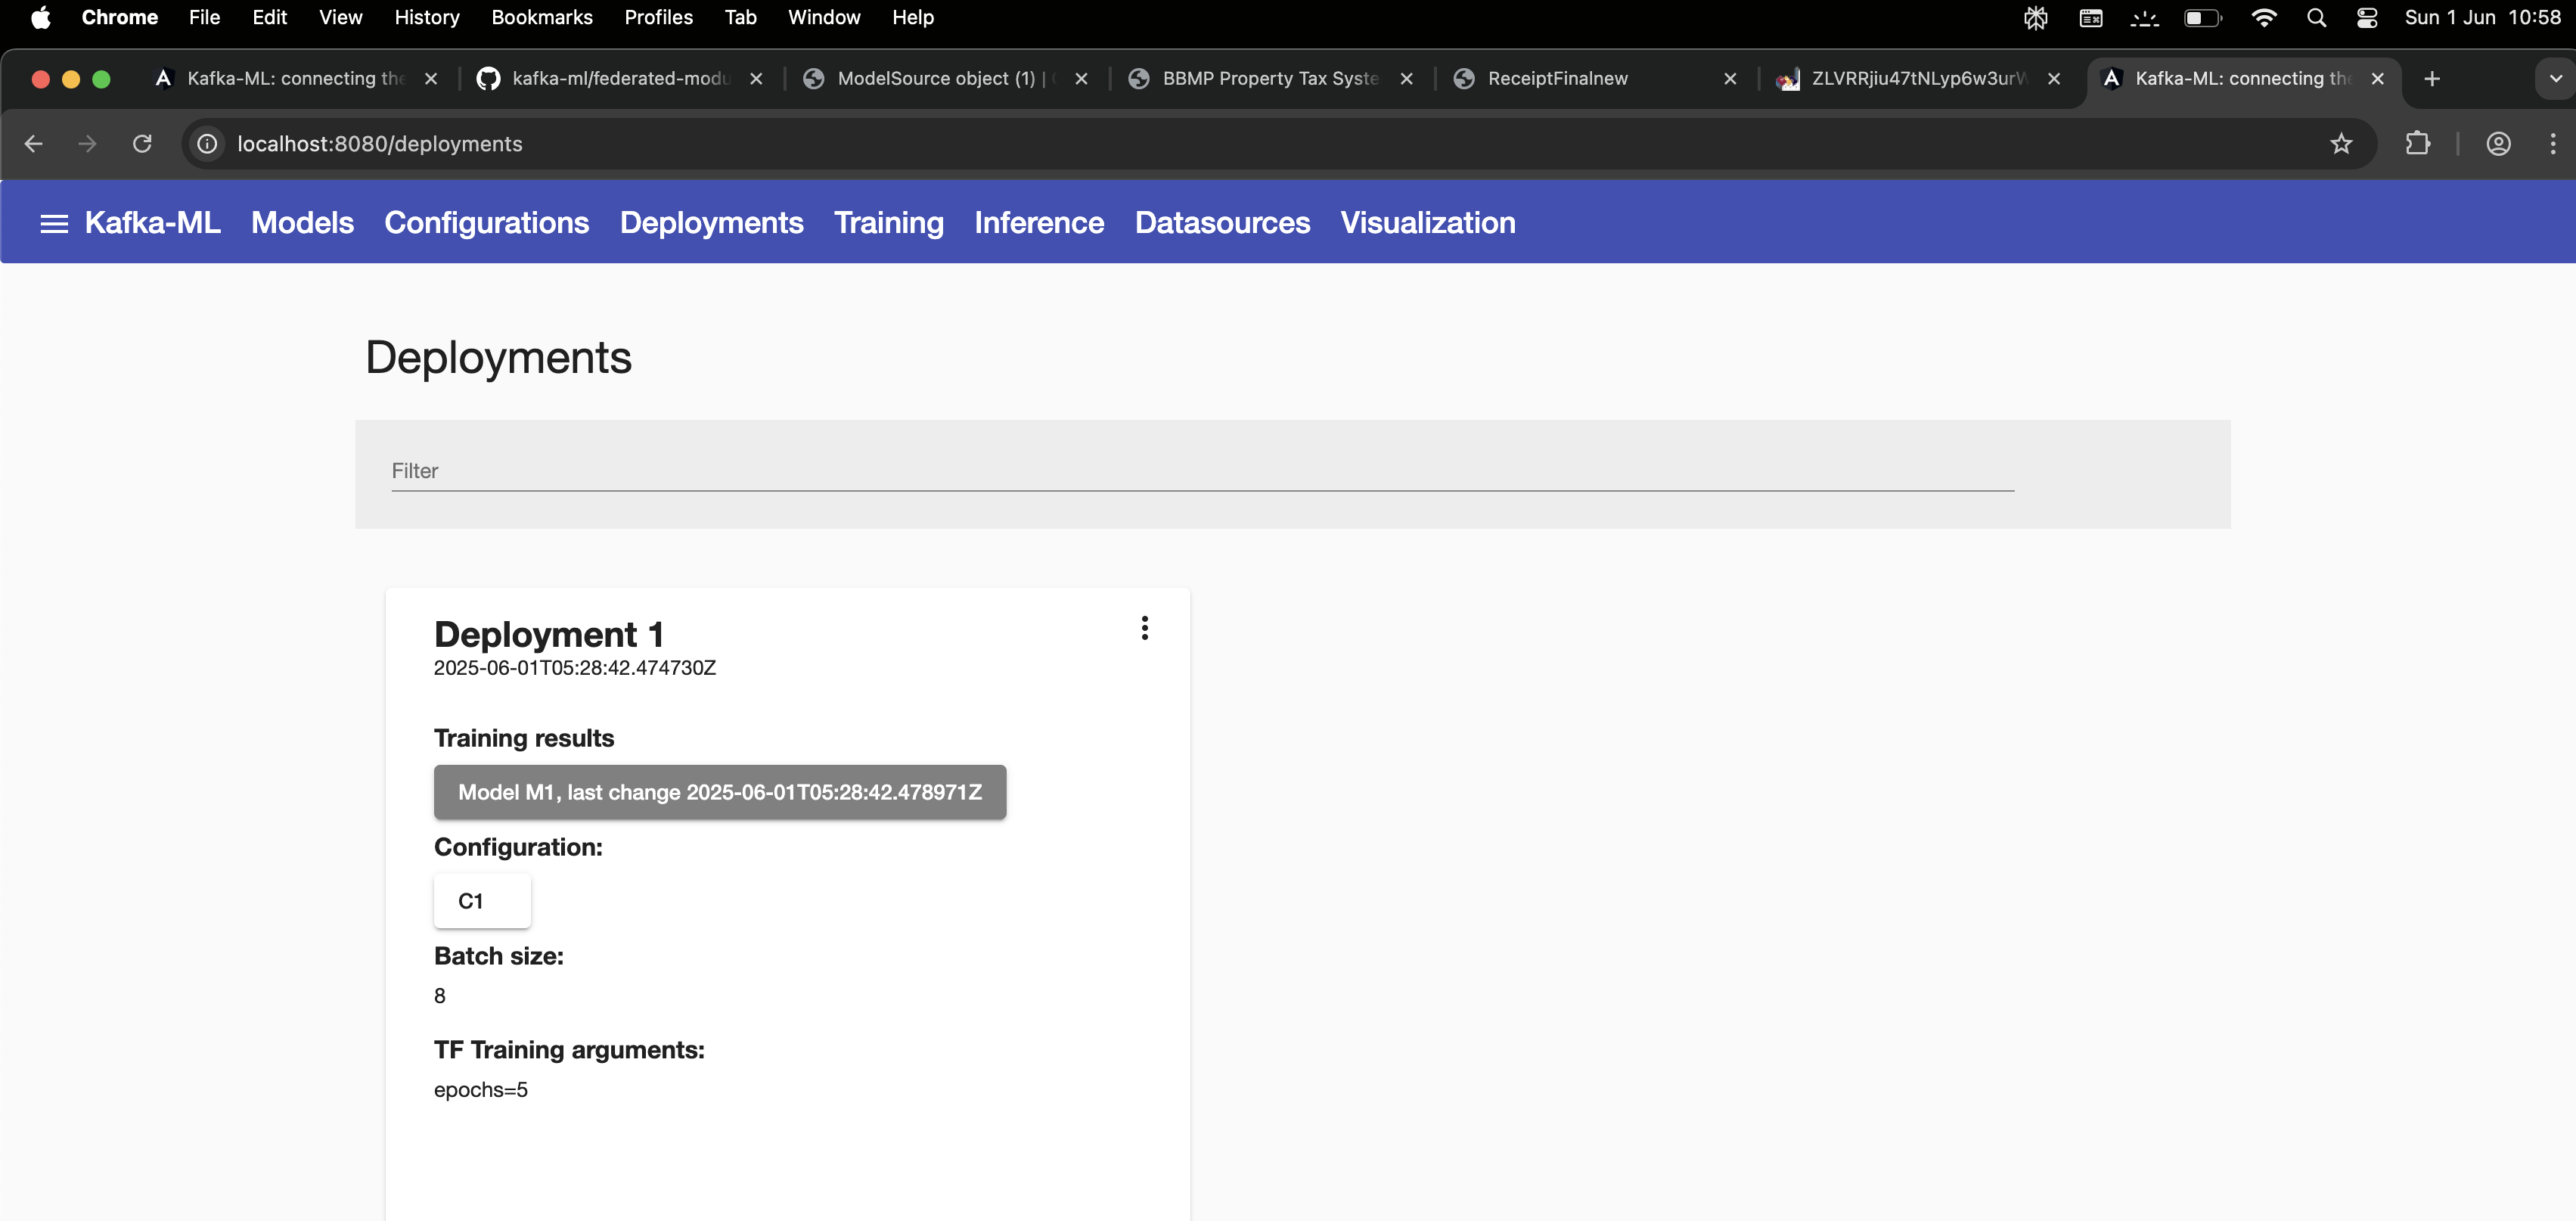
\includegraphics[width=\linewidth]{MWP-Project Report Template - BD-ML-June25/screenshots_classic/7a_deployment_created.png}
                \caption{Created Deployment}
            \end{subfigure} \\
            % Second row
            \begin{subfigure}{0.5\textwidth}
                \centering
                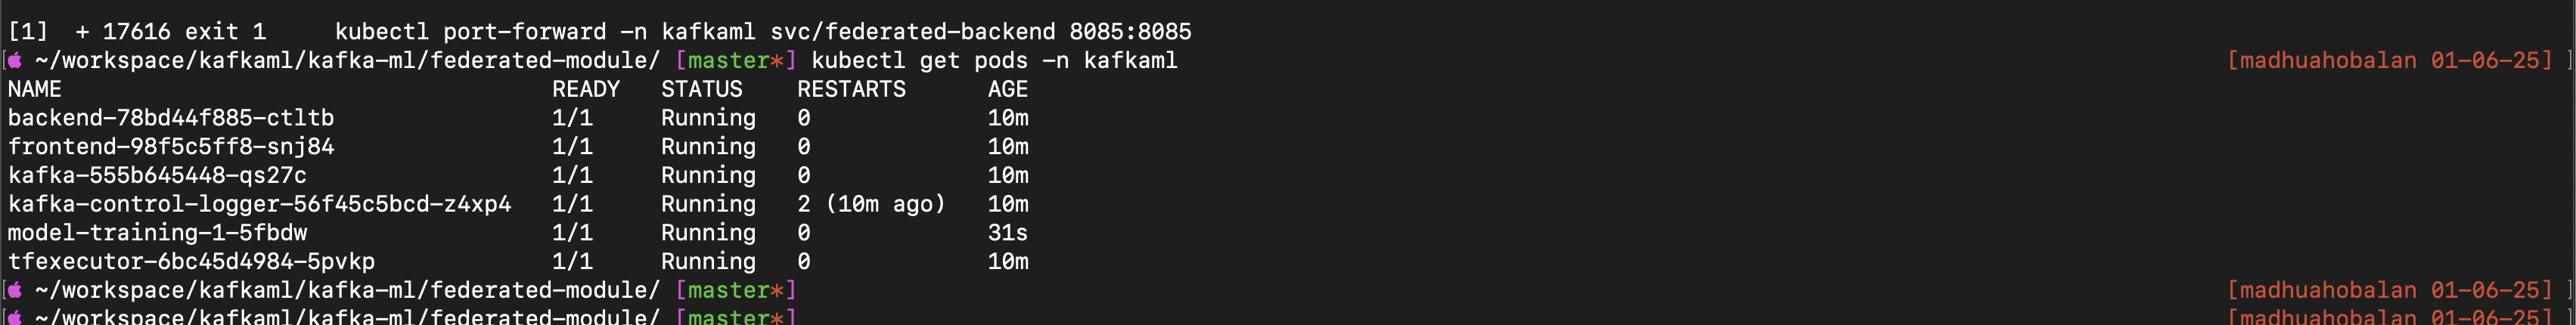
\includegraphics[width=\linewidth]{MWP-Project Report Template - BD-ML-June25/screenshots_classic/8_Deployment_Pod_Running.png}
                \caption{Training Job For Deployment}
            \end{subfigure} &
            \begin{minipage}{0.48\textwidth}
                % Empty cell for grid alignment
            \end{minipage}
        \end{tabular}
    \end{adjustbox}
    \vskip\baselineskip
    \caption{Deploy Model and Create Training Job}
    \label{fig:collage3}
\end{figure}




    \item \textbf{Model Training:} The model was then trained using the MNIST dataset. The Kafka-ML frontend provided an interface to initiate and monitor this training process. A sample image for this process is given in Fig. \ref{fig:collage4}.
    % Placeholder for a screenshot of training process/completion
\begin{figure}[h!]
    \centering
    \begin{adjustbox}{bgcolor=gray!20, padding=0.7em, margin=1ex}
        \begin{subfigure}{0.5\textwidth}
            \centering
            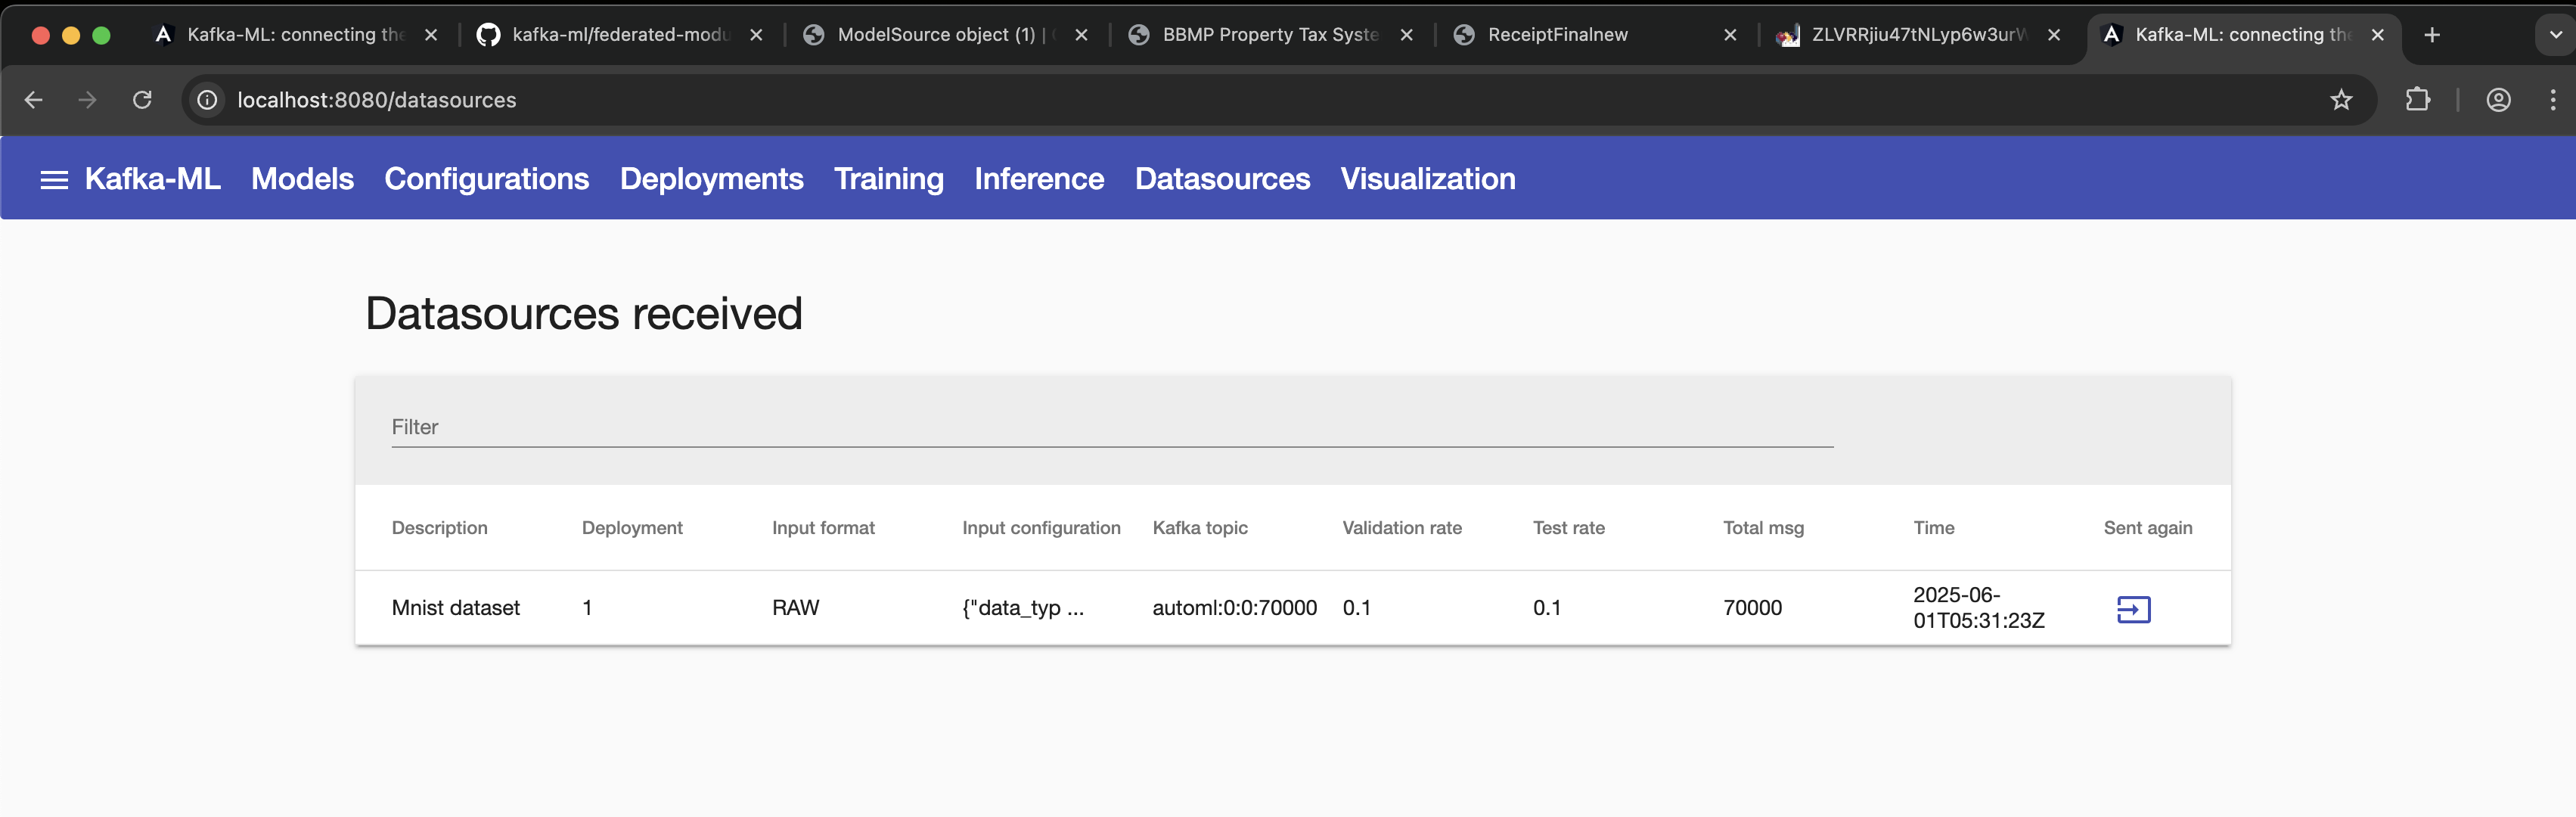
\includegraphics[width=\linewidth]{MWP-Project Report Template - BD-ML-June25/screenshots_classic/9_MNIST_Data_Injected.png}
            \caption{Data Injection}
        \end{subfigure}
        \hfill
        \begin{subfigure}{0.5\textwidth}
            \centering
            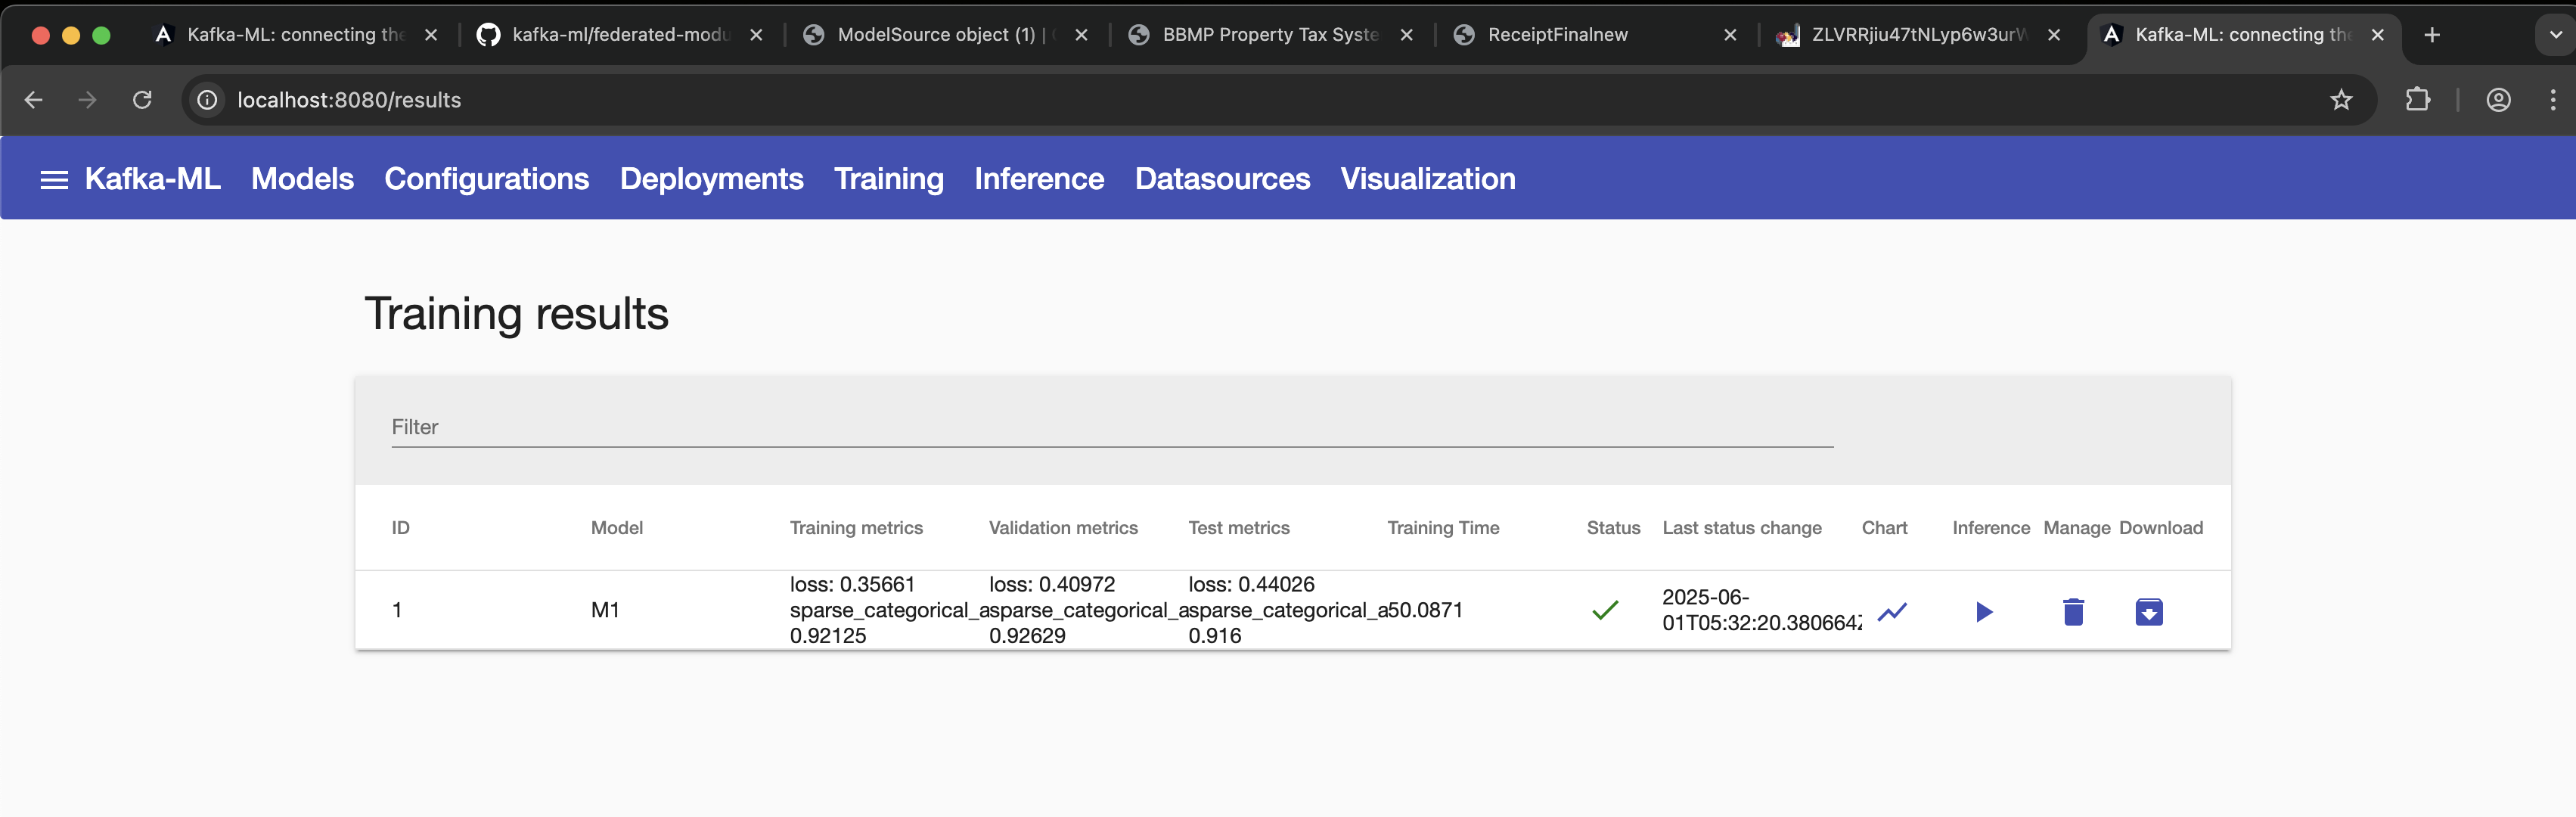
\includegraphics[width=\linewidth]{MWP-Project Report Template - BD-ML-June25/screenshots_classic/10_Model_Training_Done.png}
            \caption{Model Training Status}
        \end{subfigure}
    \end{adjustbox}
    \vskip\baselineskip
    \caption{Data Injection and Monitoring Training.}
    \label{fig:collage4}
\end{figure}


    \item \textbf{Creating Inference Engine and Running Inference:} After successful training, an inference engine (see Fig. \ref{fig:collage5}) was created from the trained model. Sample MNIST data was then used to run inference, testing the model's ability to predict handwritten digits.
    % Placeholder for a screenshot of inference setup or input
\begin{figure}[h!]
    \centering
    \begin{adjustbox}{bgcolor=gray!20, padding=0.7em, margin=1ex}
        \begin{subfigure}{0.5\textwidth}
            \centering
            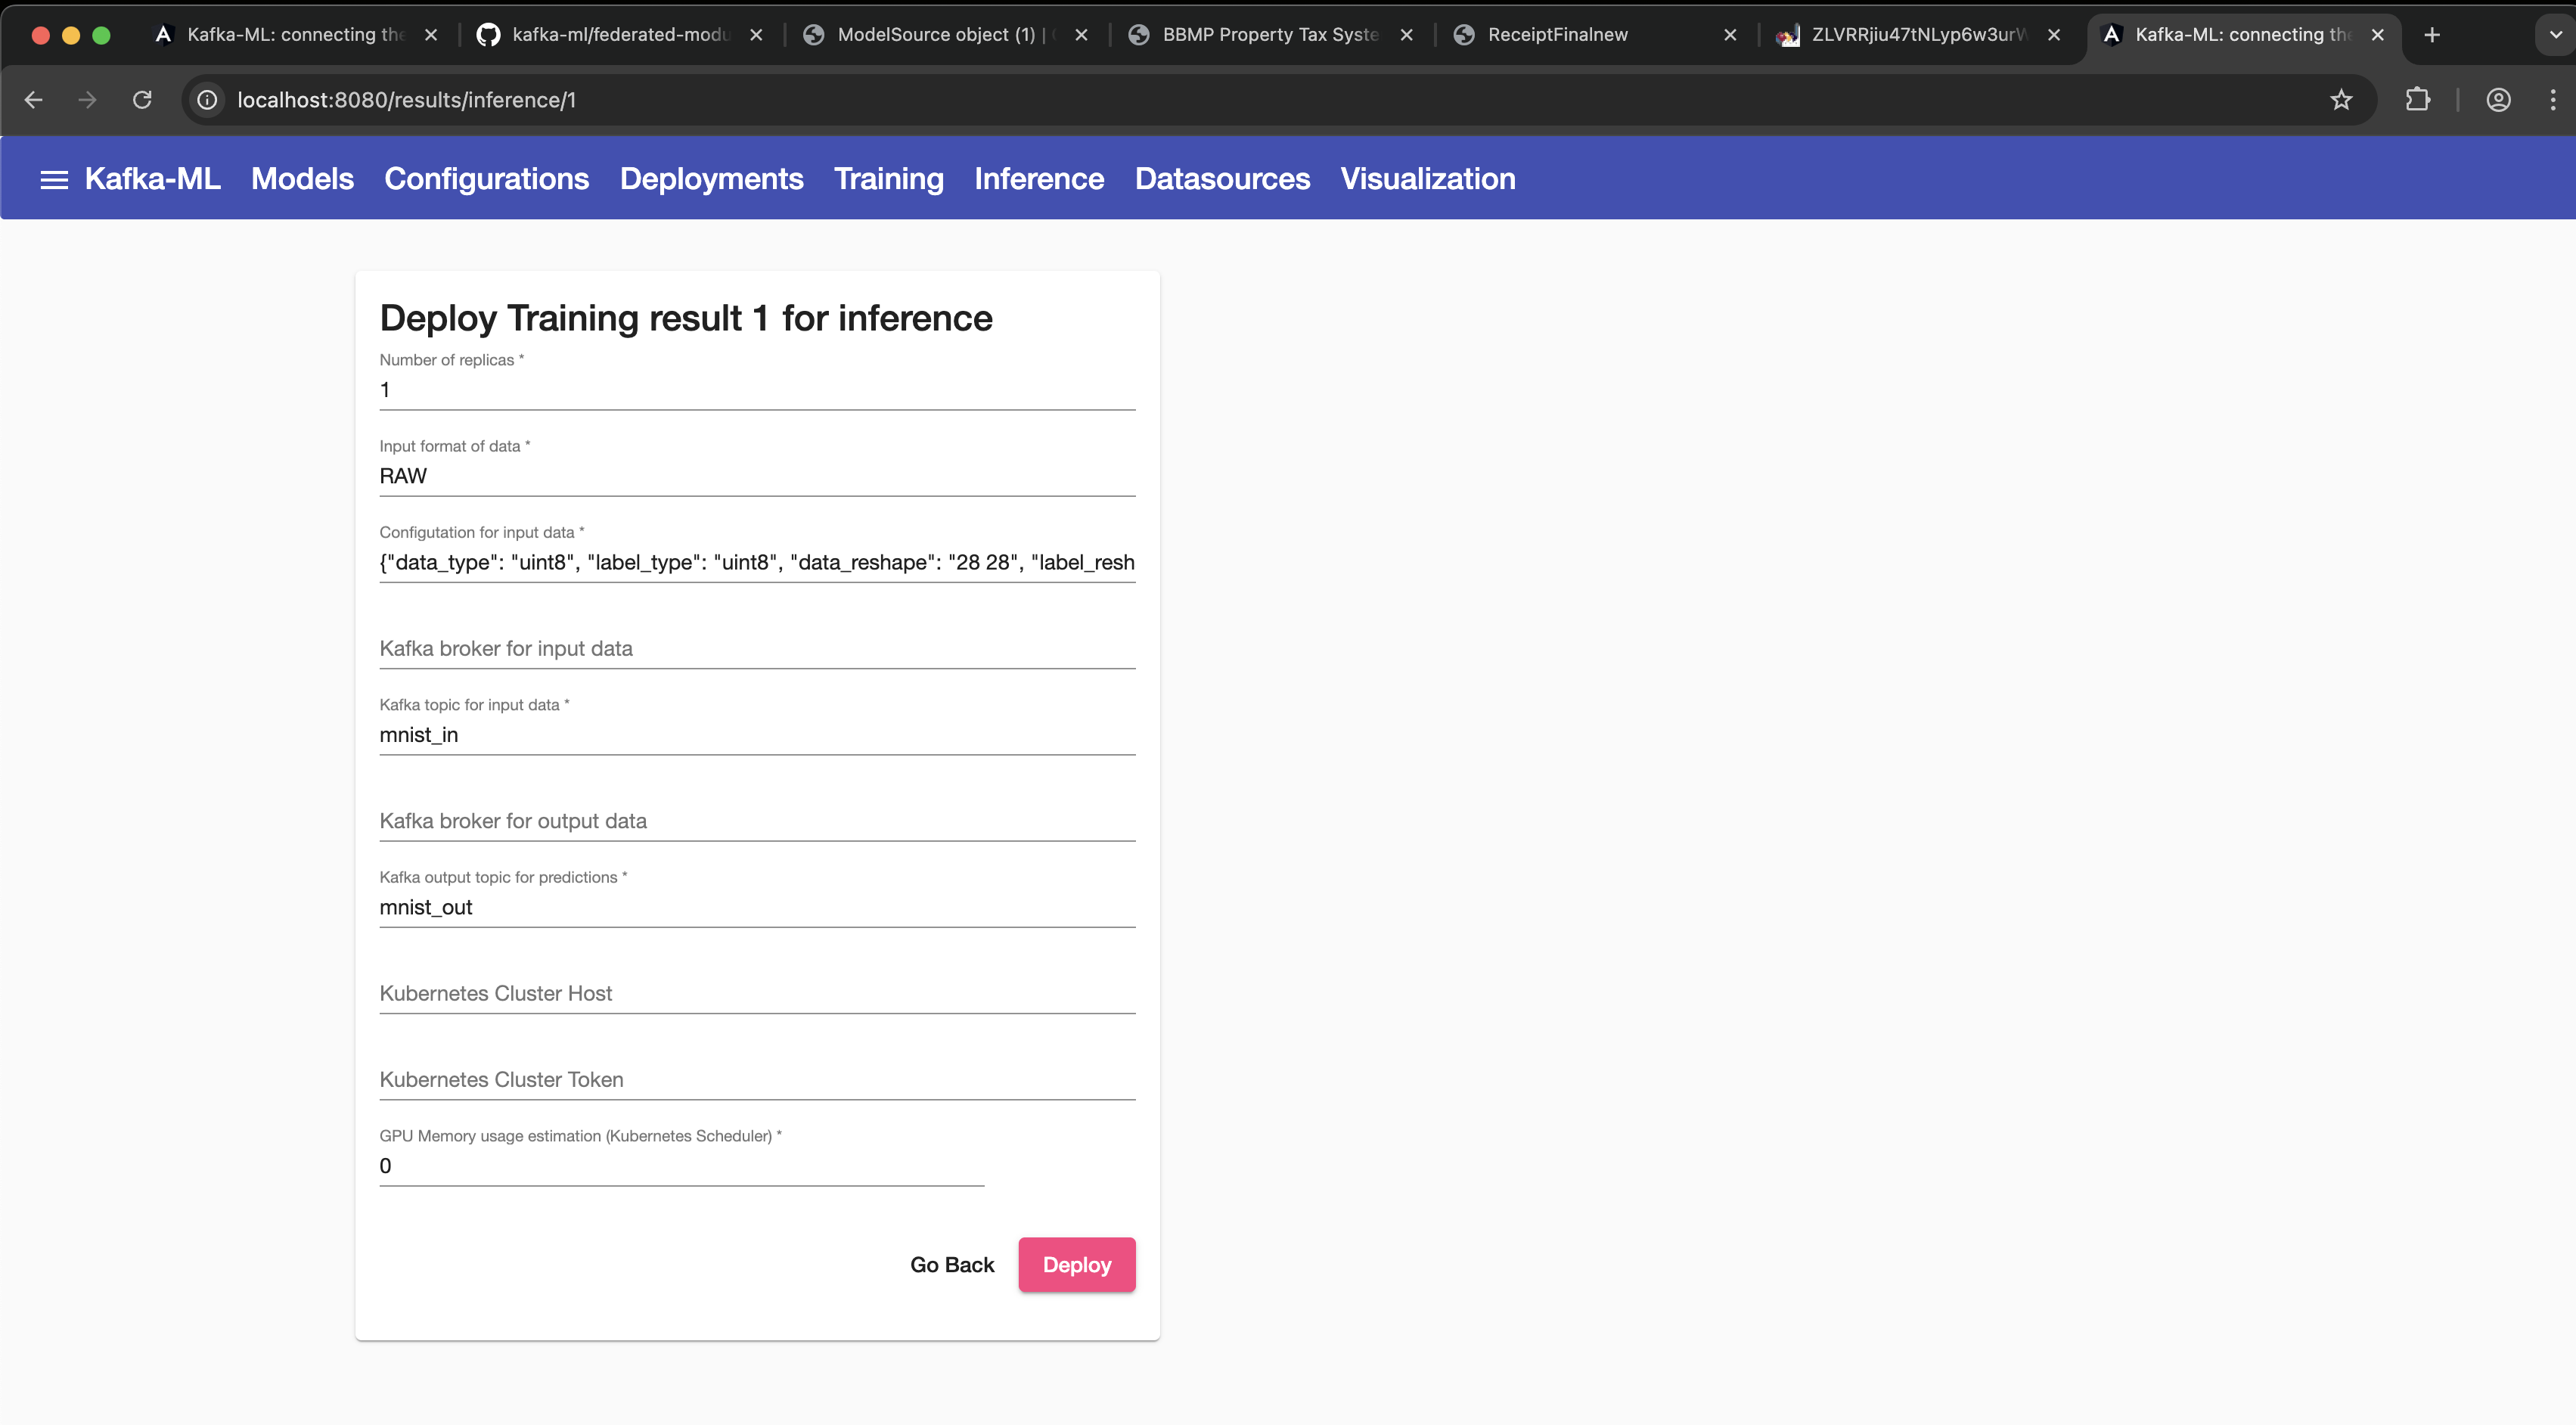
\includegraphics[width=\linewidth]{MWP-Project Report Template - BD-ML-June25/screenshots_classic/11_Inference_Engine.png}
            \caption{Inference Setup}
        \end{subfigure}
        \hfill
        \begin{subfigure}{0.5\textwidth}
            \centering
            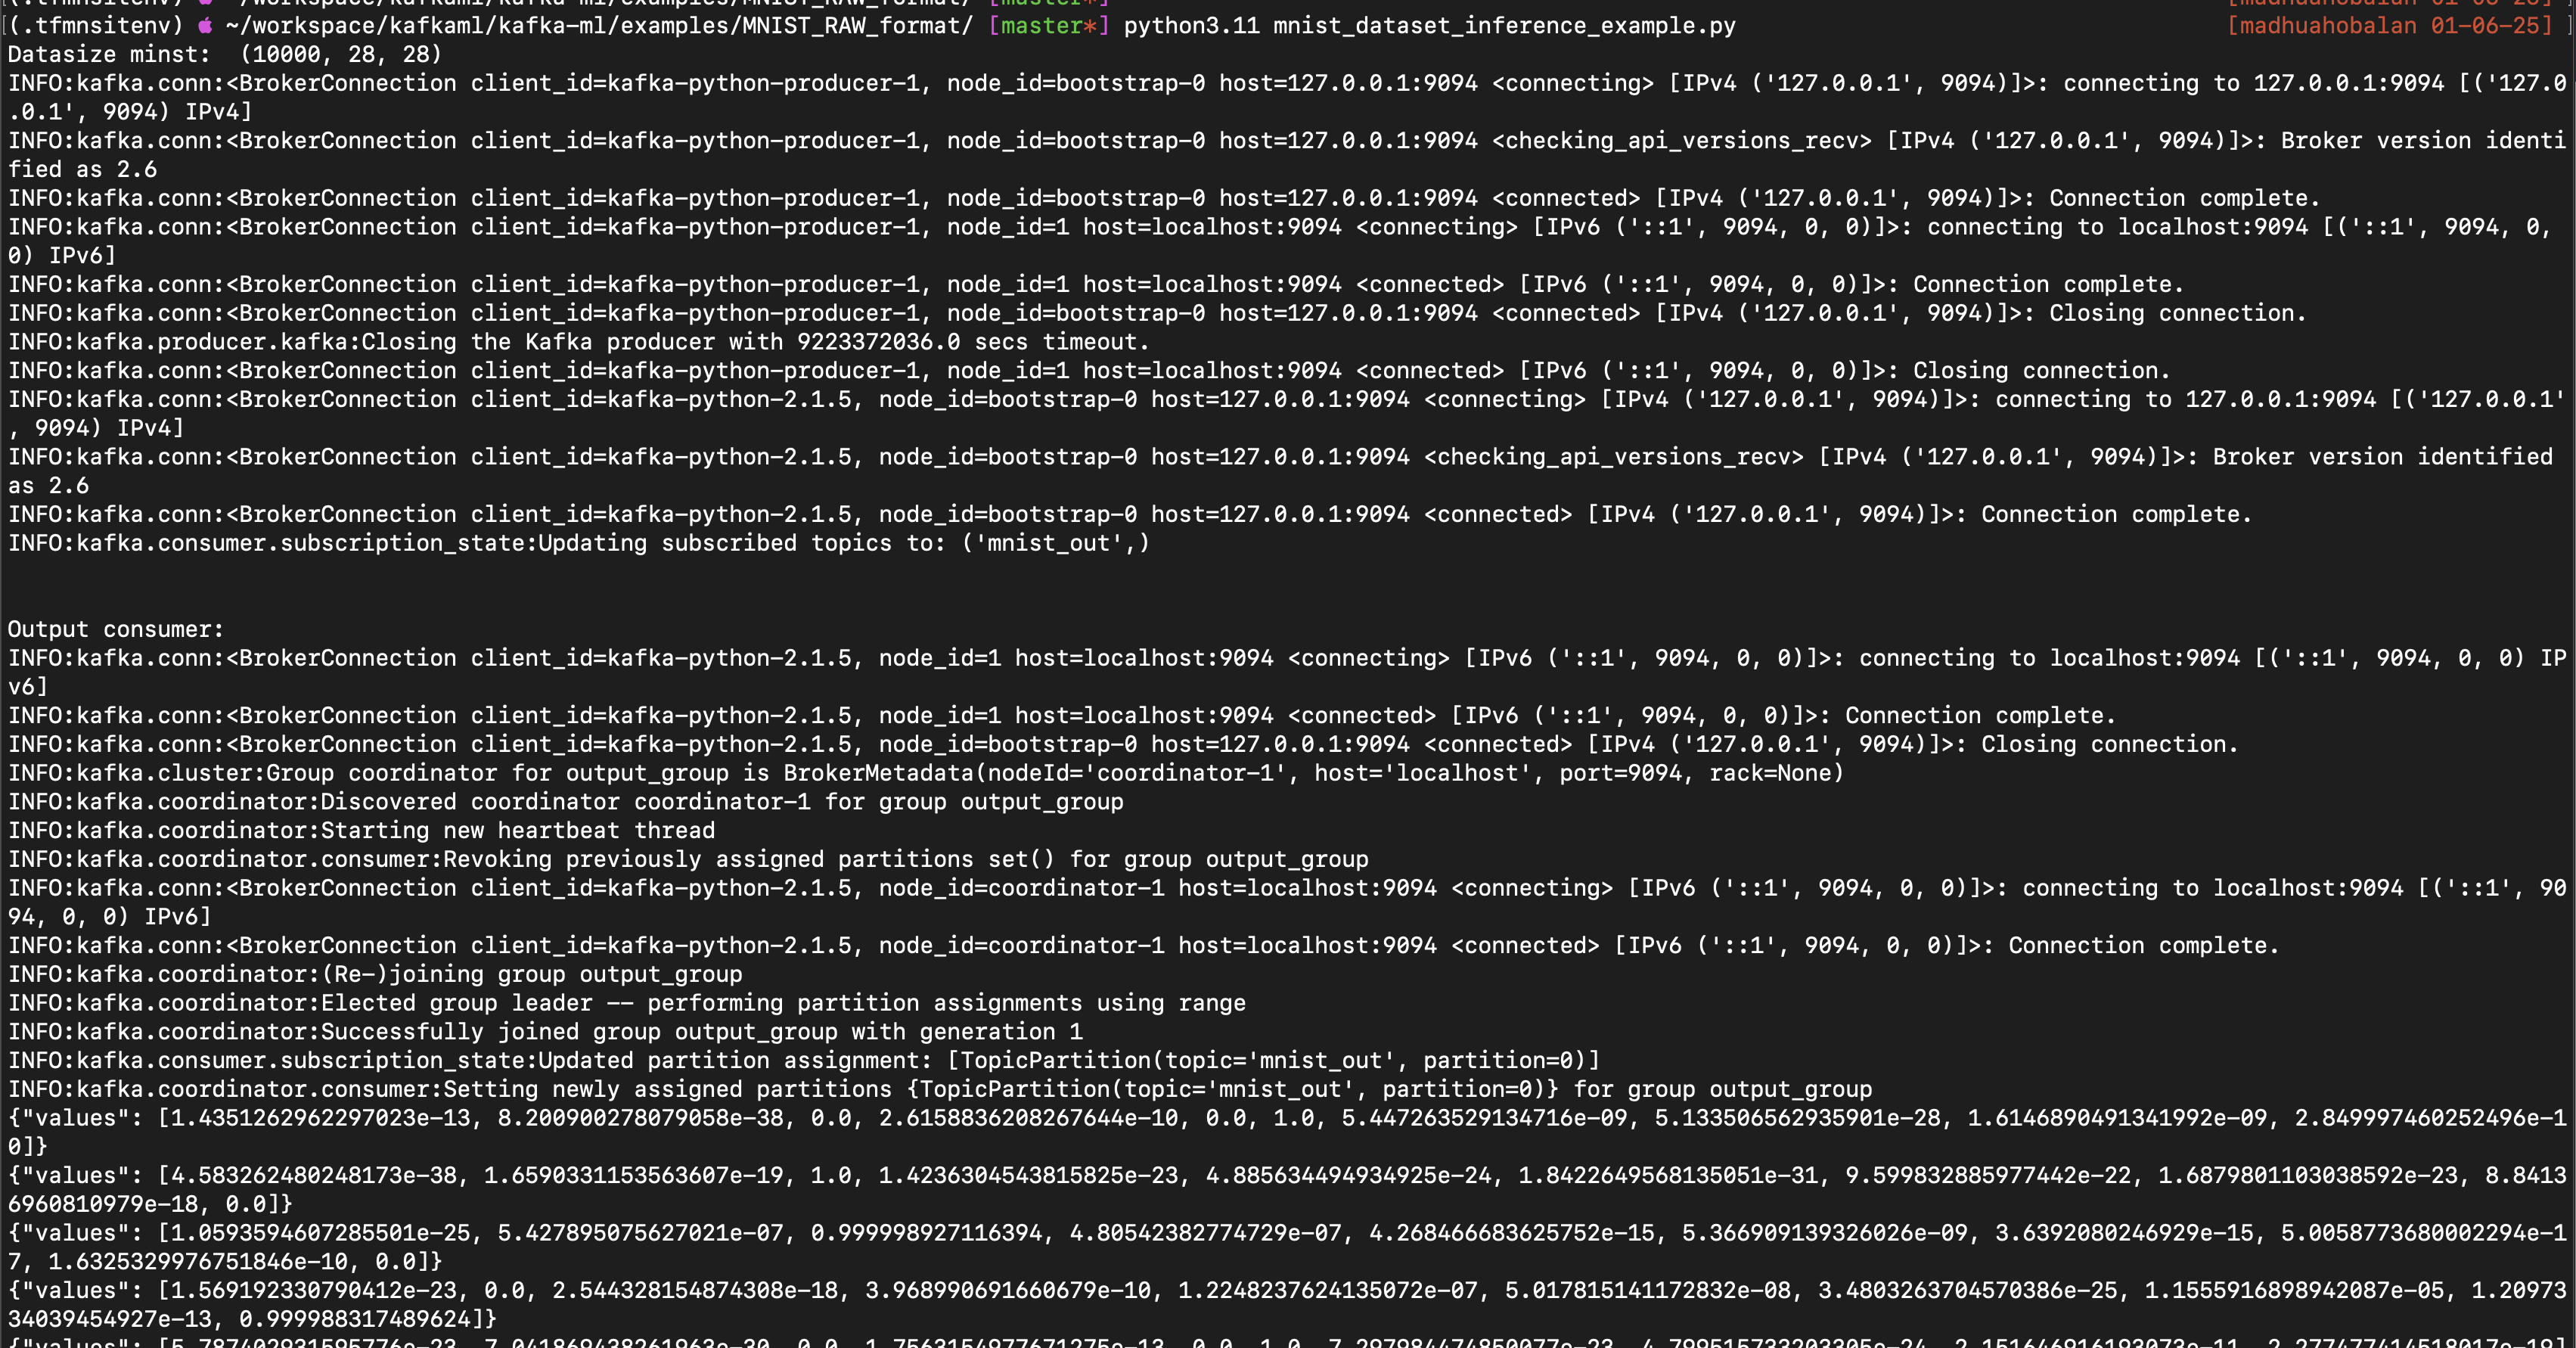
\includegraphics[width=\linewidth]{MWP-Project Report Template - BD-ML-June25/screenshots_classic/12_Send_Inference_Data.png}
            \caption{Inference Data Input}
        \end{subfigure}
    \end{adjustbox}
    \vskip\baselineskip
    \caption{Inference Engine Setup and Data Input}
    \label{fig:collage5}
\end{figure}


    \item \textbf{Visualization of Inference Results:} The results from the inference process were visualized (see Fig. \ref{fig:inference_results6}), typically showing the input digit image and the model's prediction. This step confirmed the successful operation of the entire pipeline from model deployment to prediction.
    % Placeholder for a screenshot of inference results visualization
    \begin{figure}[h!]
        \centering
         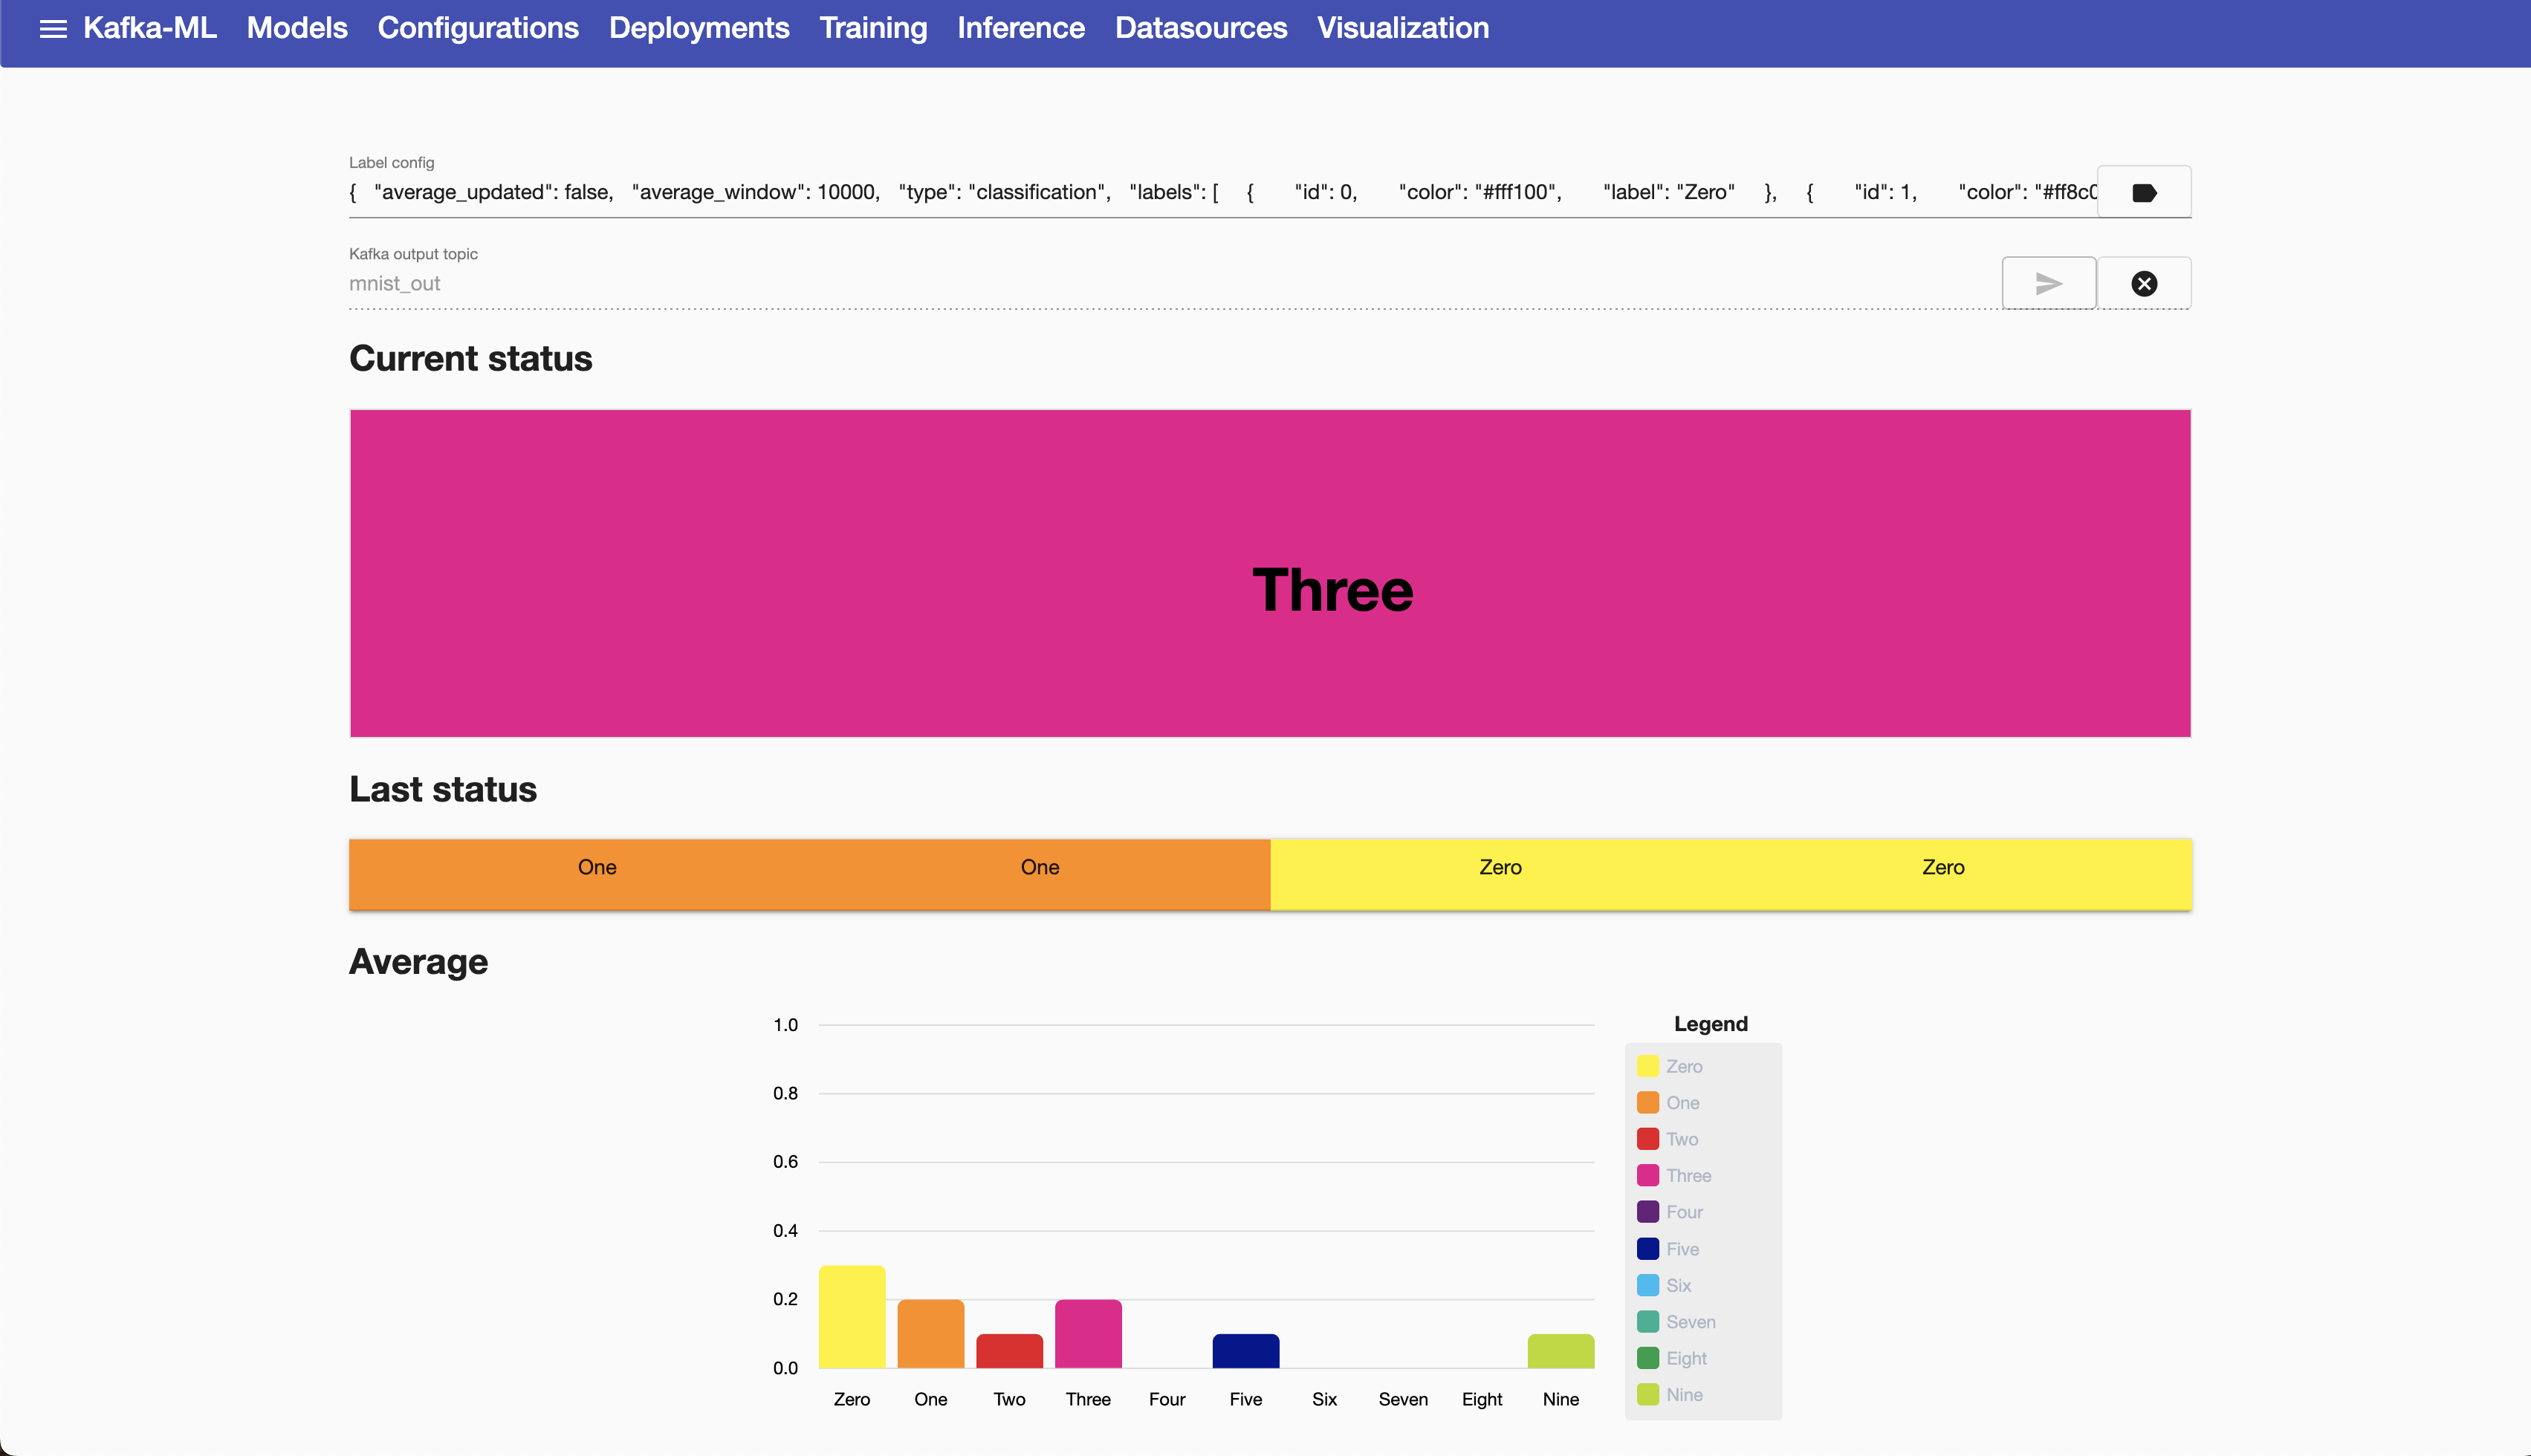
\includegraphics[width=0.7\textwidth]{MWP-Project Report Template - BD-ML-June25/screenshots_classic/13_Visualisation.png}
       
        \caption{Visualization of inference results on sample MNIST digits.}
        \label{fig:inference_results6}
    \end{figure}
\end{enumerate}

The successful execution of these steps validated the core functionalities of the Kafka-ML classic model architecture and confirmed that the local deployment environment was correctly configured for further development and experimentation.


\subsection{Setup and Initial Run of Federated Learning Module (Non-Distributed)}
\label{subsec:federated_setup_non_distributed}

Following the successful validation of the classic model architecture, the next phase focused on setting up the federated learning module. For this initial stage, the setup was configured for non-distributed datasets to test the core components of the federated backend, model control, and data control mechanisms.

\paragraph{Dockerization and Kubernetes Deployment for Federated Module}
Similar to the classic setup, the federated learning module components were prepared for a containerized deployment as shown in Fig. \ref{fig:collage7}:
\begin{itemize}
    \item Docker images for the federated learning specific components (e.g., Federated Backend, Federated Model Control Logger, Federated Data Control Logger, Federated Model Training) were built. This process included integrating necessary libraries and adjustments for the federated workflow.
    \item These images were subsequently pushed to a Docker registry.
    \item Kustomization files were adapted and created to define the deployment configuration for the federated learning services on the local Minikube Kubernetes cluster.
    \item The federated learning module was then deployed to the Minikube cluster.
\end{itemize}

\begin{figure}[h!]
    \centering
    \begin{adjustbox}{bgcolor=gray!20, padding=0.7em, margin=1ex}
        \begin{tabular}{cc}
            % First row
            \begin{subfigure}{0.48\textwidth}
                \centering
                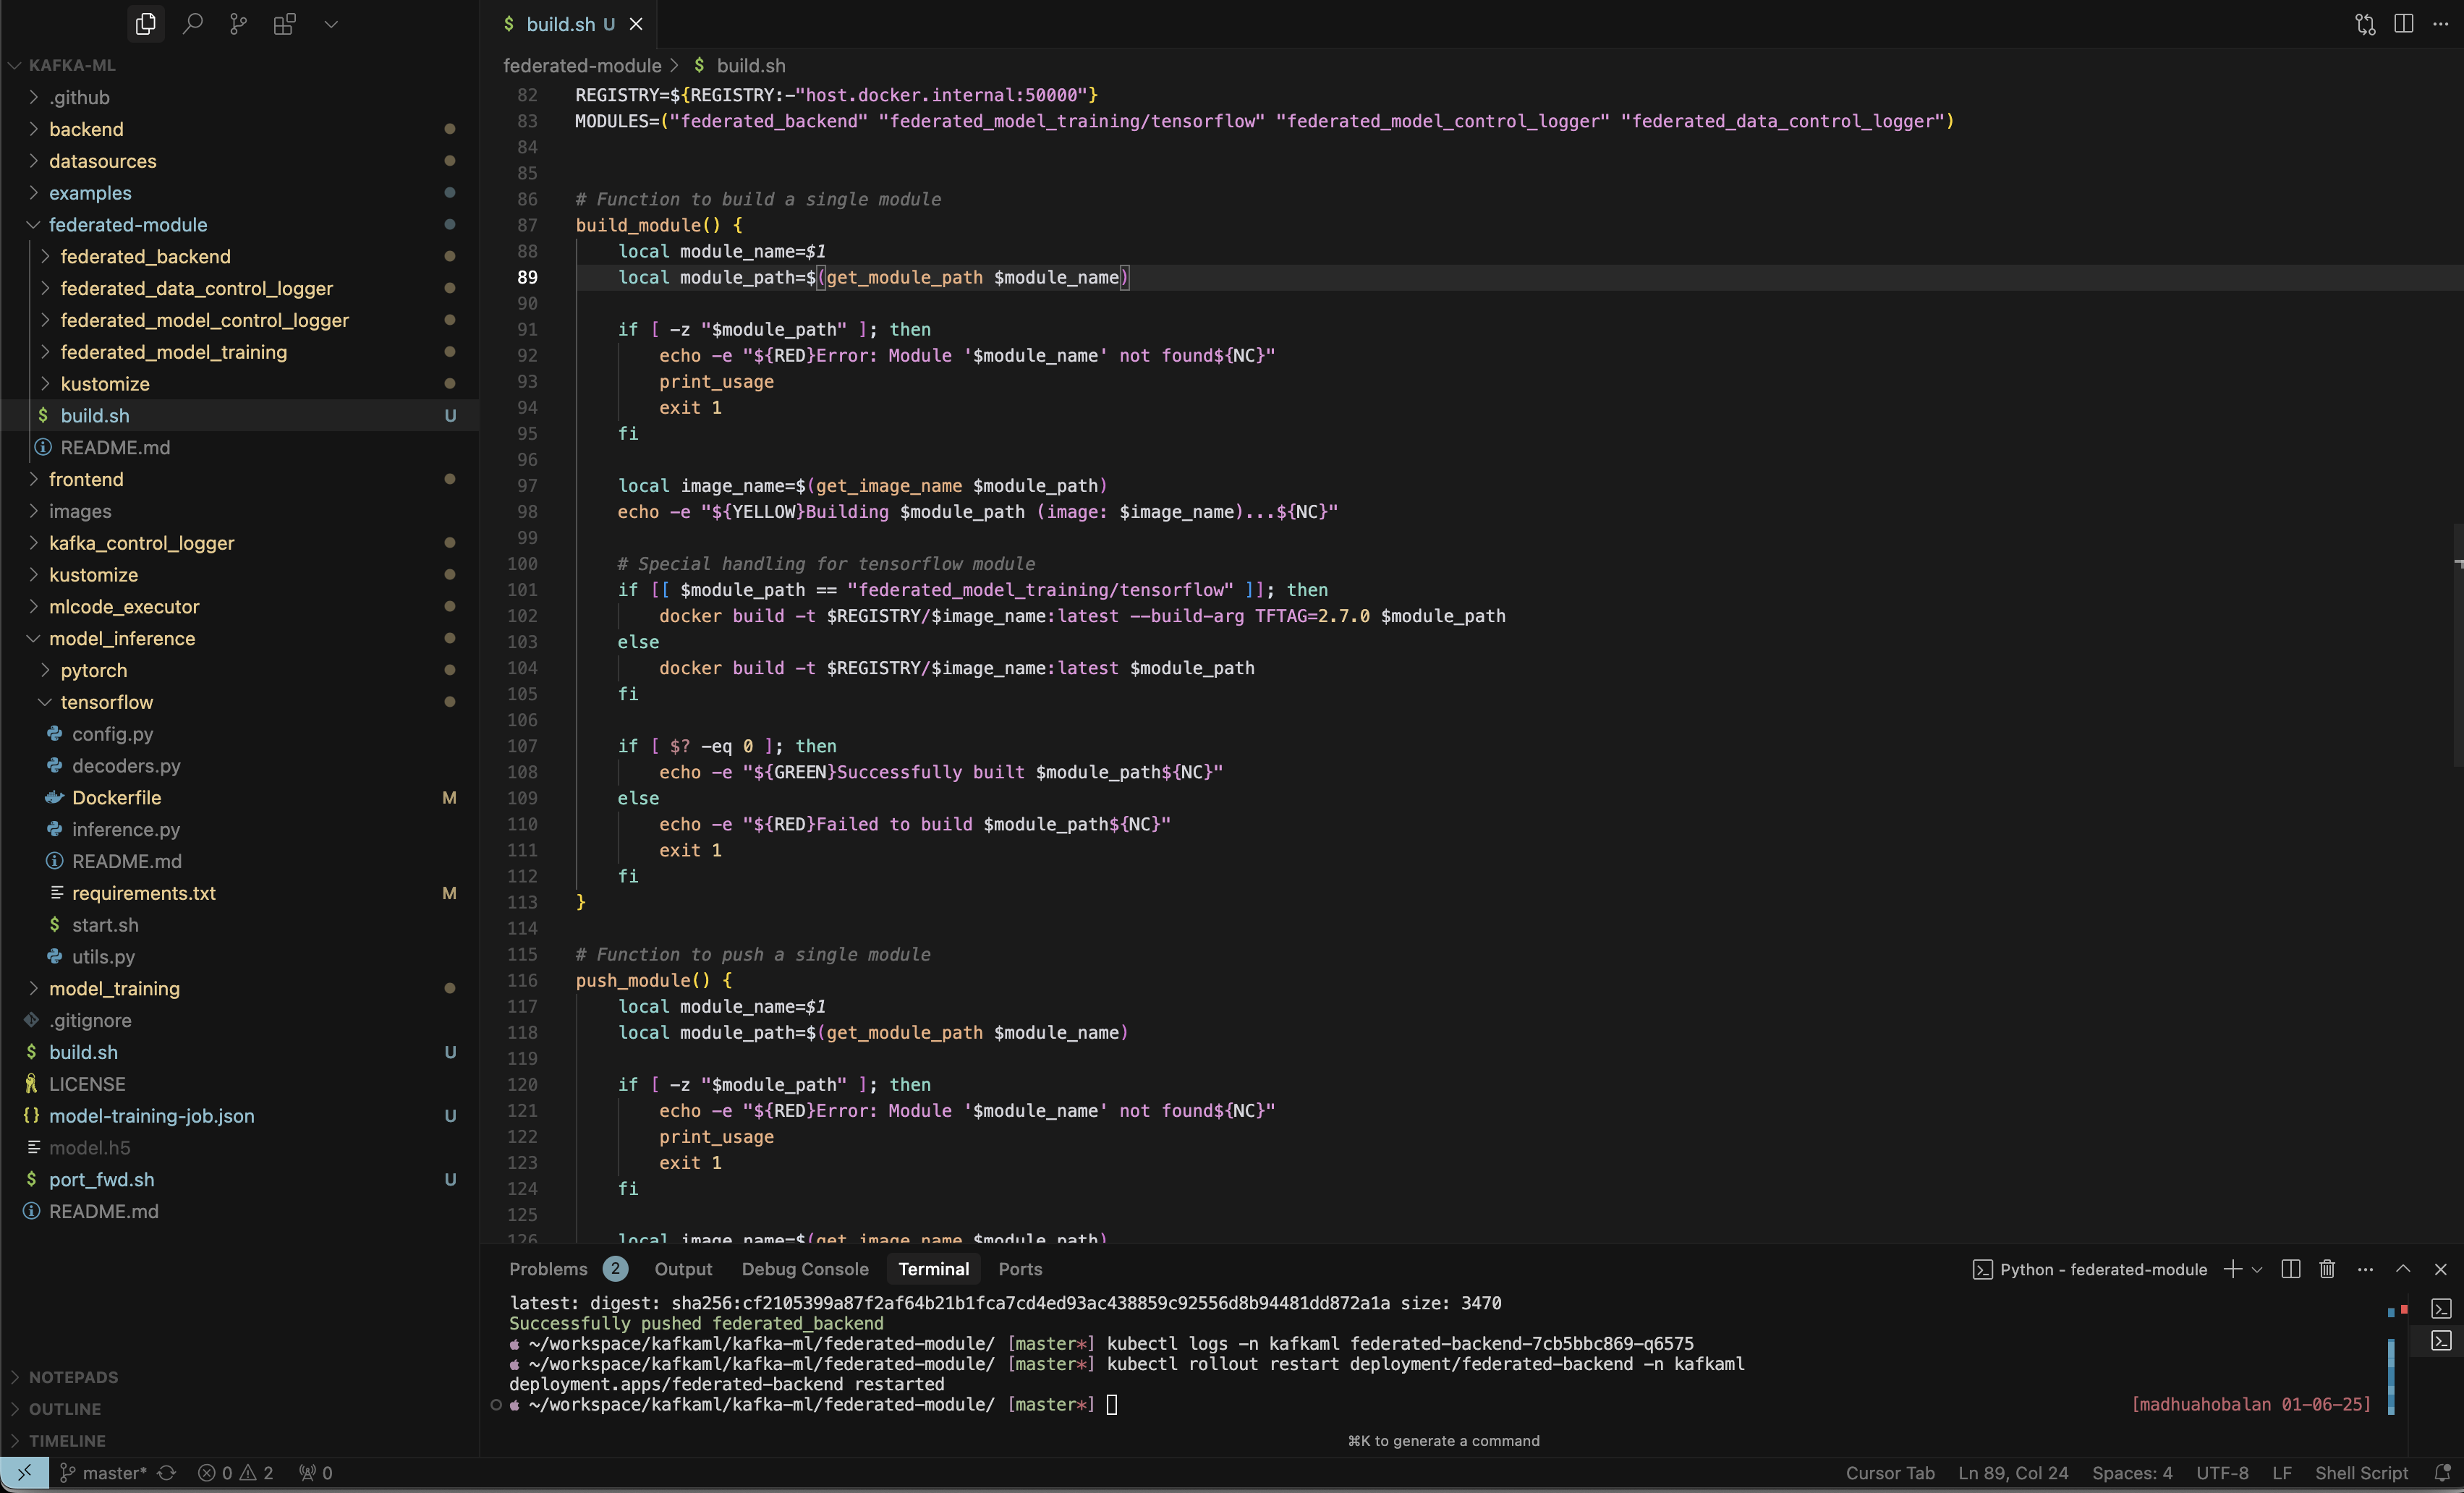
\includegraphics[width=\linewidth]{MWP-Project Report Template - BD-ML-June25/screenshots_federated/1_build_script.png}
                \caption{Build Script}
            \end{subfigure} &
            \begin{subfigure}{0.48\textwidth}
                \centering
                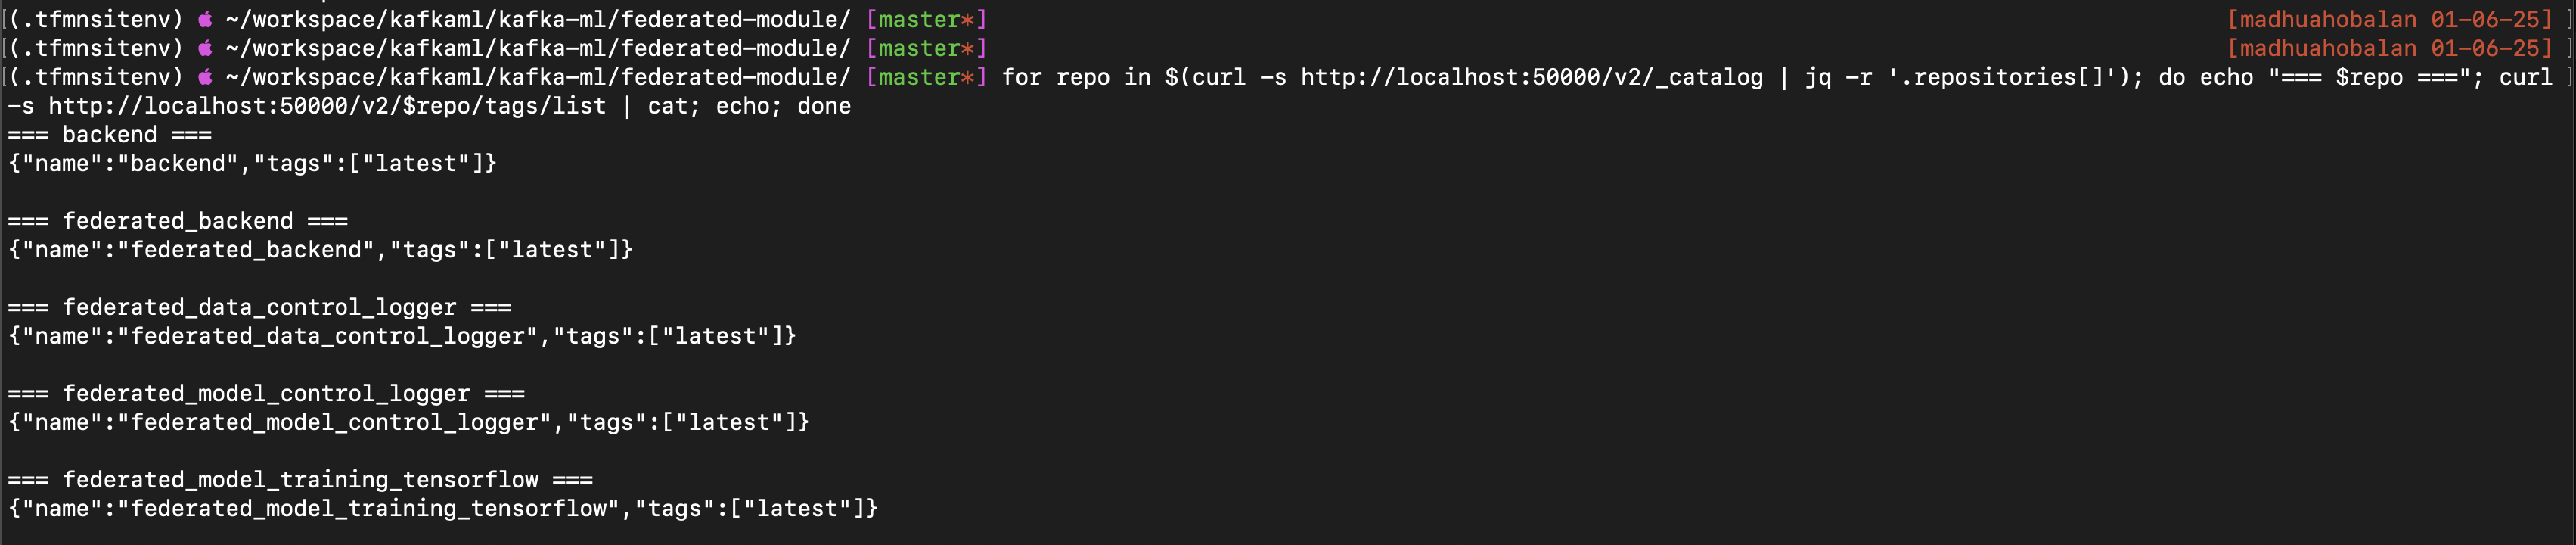
\includegraphics[width=\linewidth]{MWP-Project Report Template - BD-ML-June25/screenshots_federated/2_Docker_Images.png}
                \caption{Docker Images}
            \end{subfigure} \\
            % Second row
            \begin{subfigure}{0.48\textwidth}
                \centering
                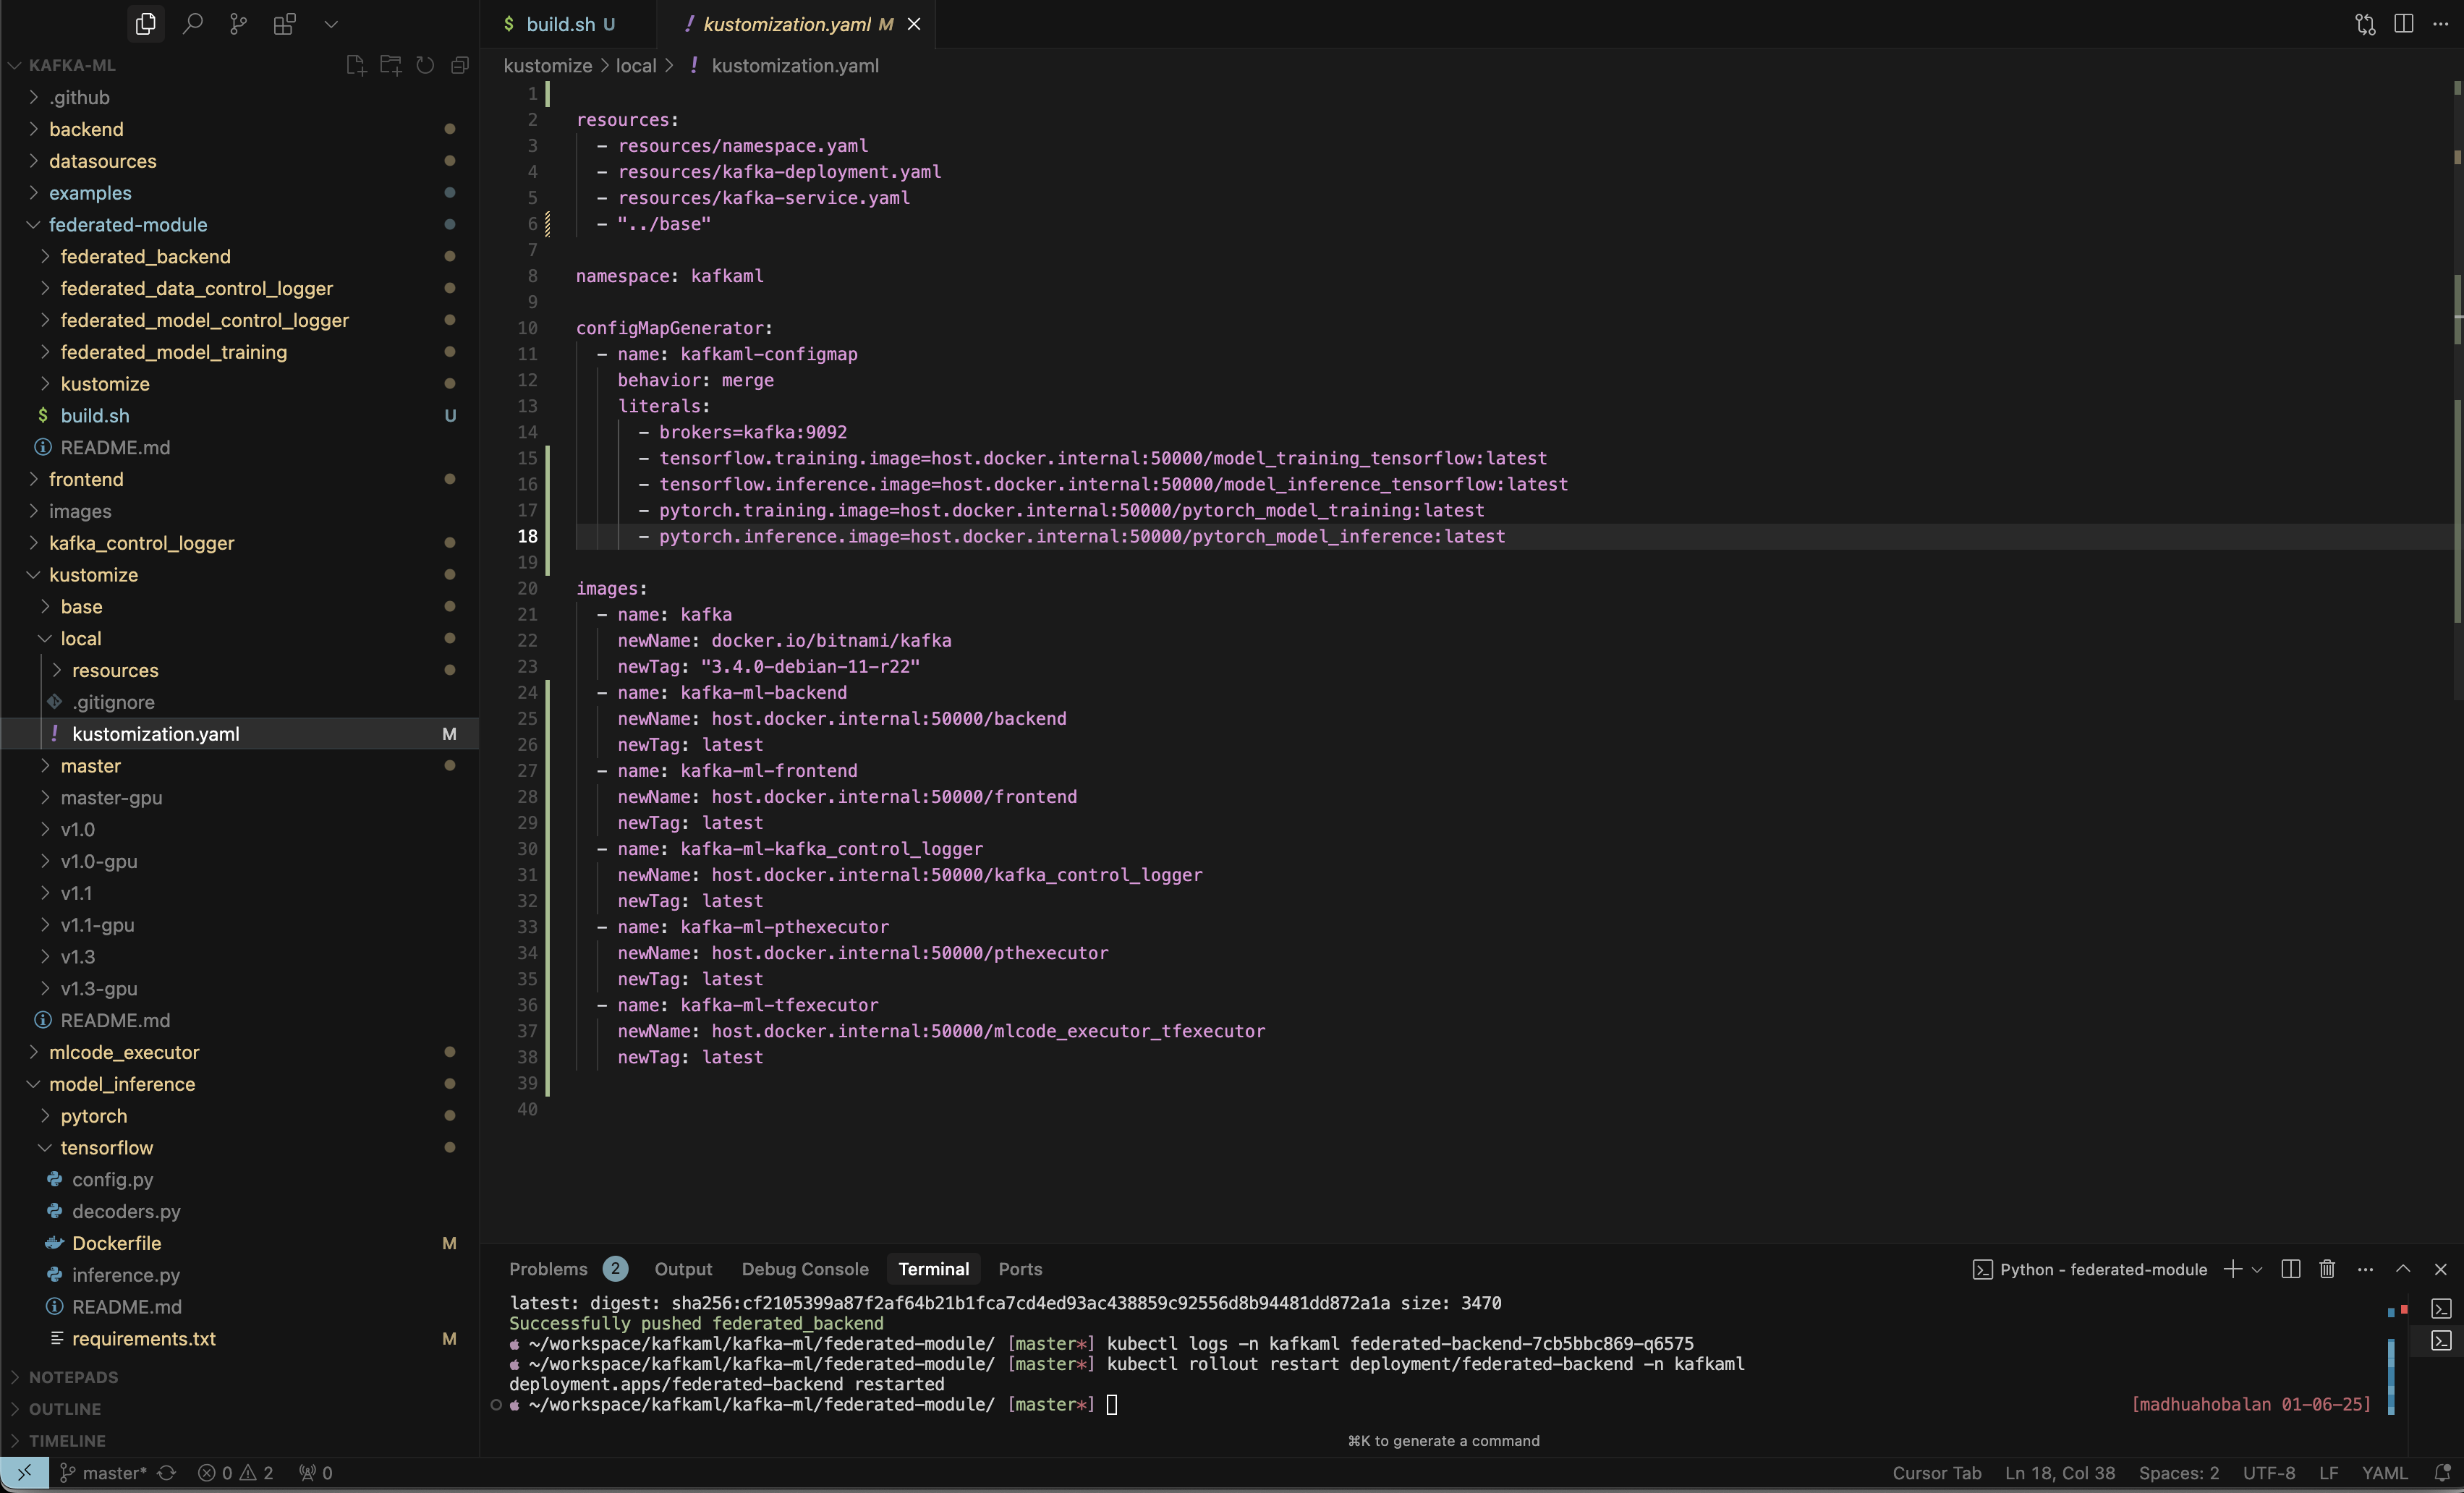
\includegraphics[width=\linewidth]{MWP-Project Report Template - BD-ML-June25/screenshots_federated/3_Deployment_Script.png}
                \caption{Deployment Script}
            \end{subfigure} &
            \begin{subfigure}{0.48\textwidth}
                \centering
                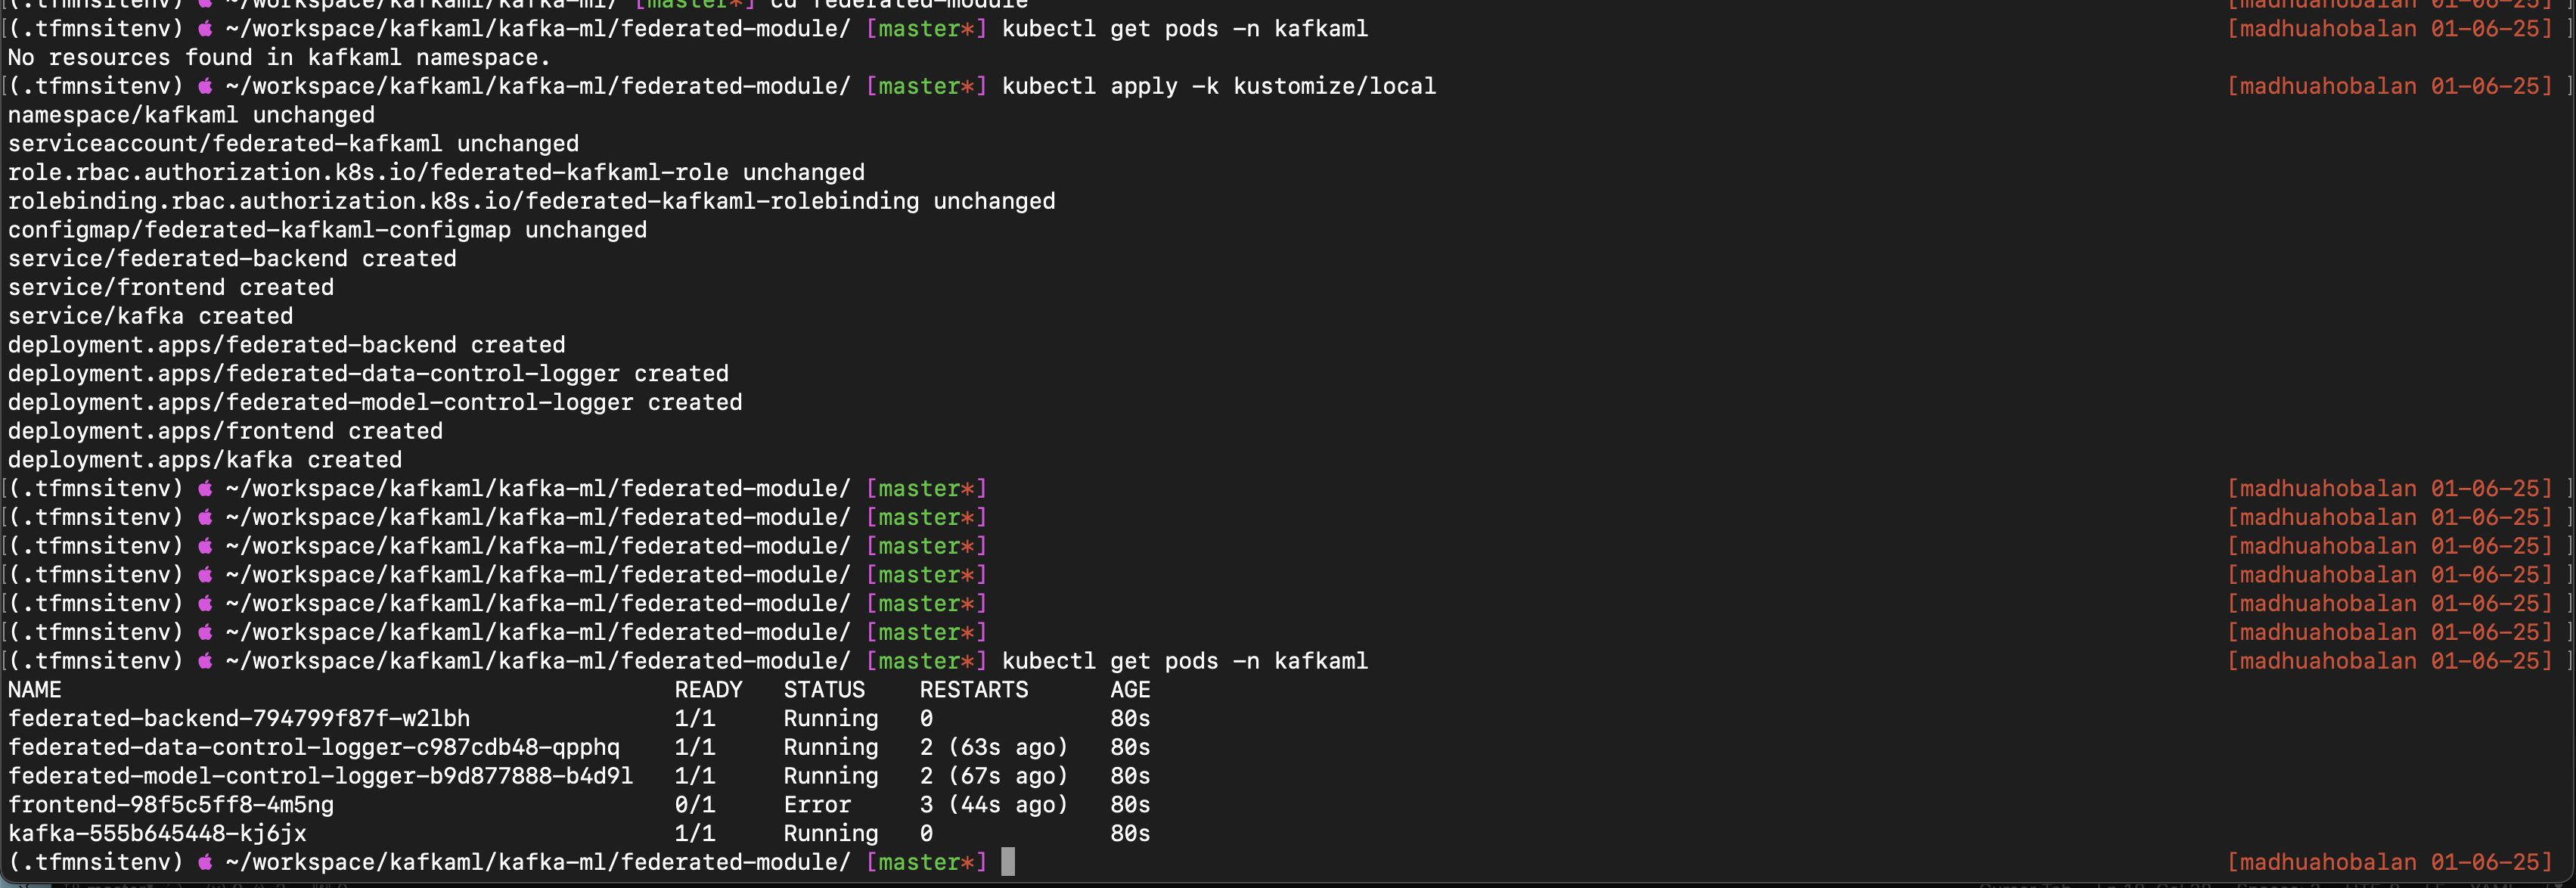
\includegraphics[width=\linewidth]{MWP-Project Report Template - BD-ML-June25/screenshots_federated/4_Running_Pods.png}
                \caption{Running Kubernetes Pods}
            \end{subfigure}
        \end{tabular}
    \end{adjustbox}
    \vskip\baselineskip
    \caption{Federated Kafka ML Build and Deploy Steps}
    \label{fig:collage7}
\end{figure}

\paragraph{Configuration via Federated Backend (Django Admin UI)}
Once the federated module was running on Minikube, the Django Admin UI, serving as part of the Federated Backend, was used to configure and initiate the federated training process:

\begin{enumerate}
    \item \textbf{Submission of Model Control Dataset:} The model control dataset, which dictates the parameters and configurations for the federated model training (e.g., model architecture, aggregation strategy), was submitted through the Django Admin UI (see Fig. \ref{fig:model_control_submission}).
    % Placeholder for a screenshot of submitting model control dataset
    \begin{figure}[h!]
        \centering
         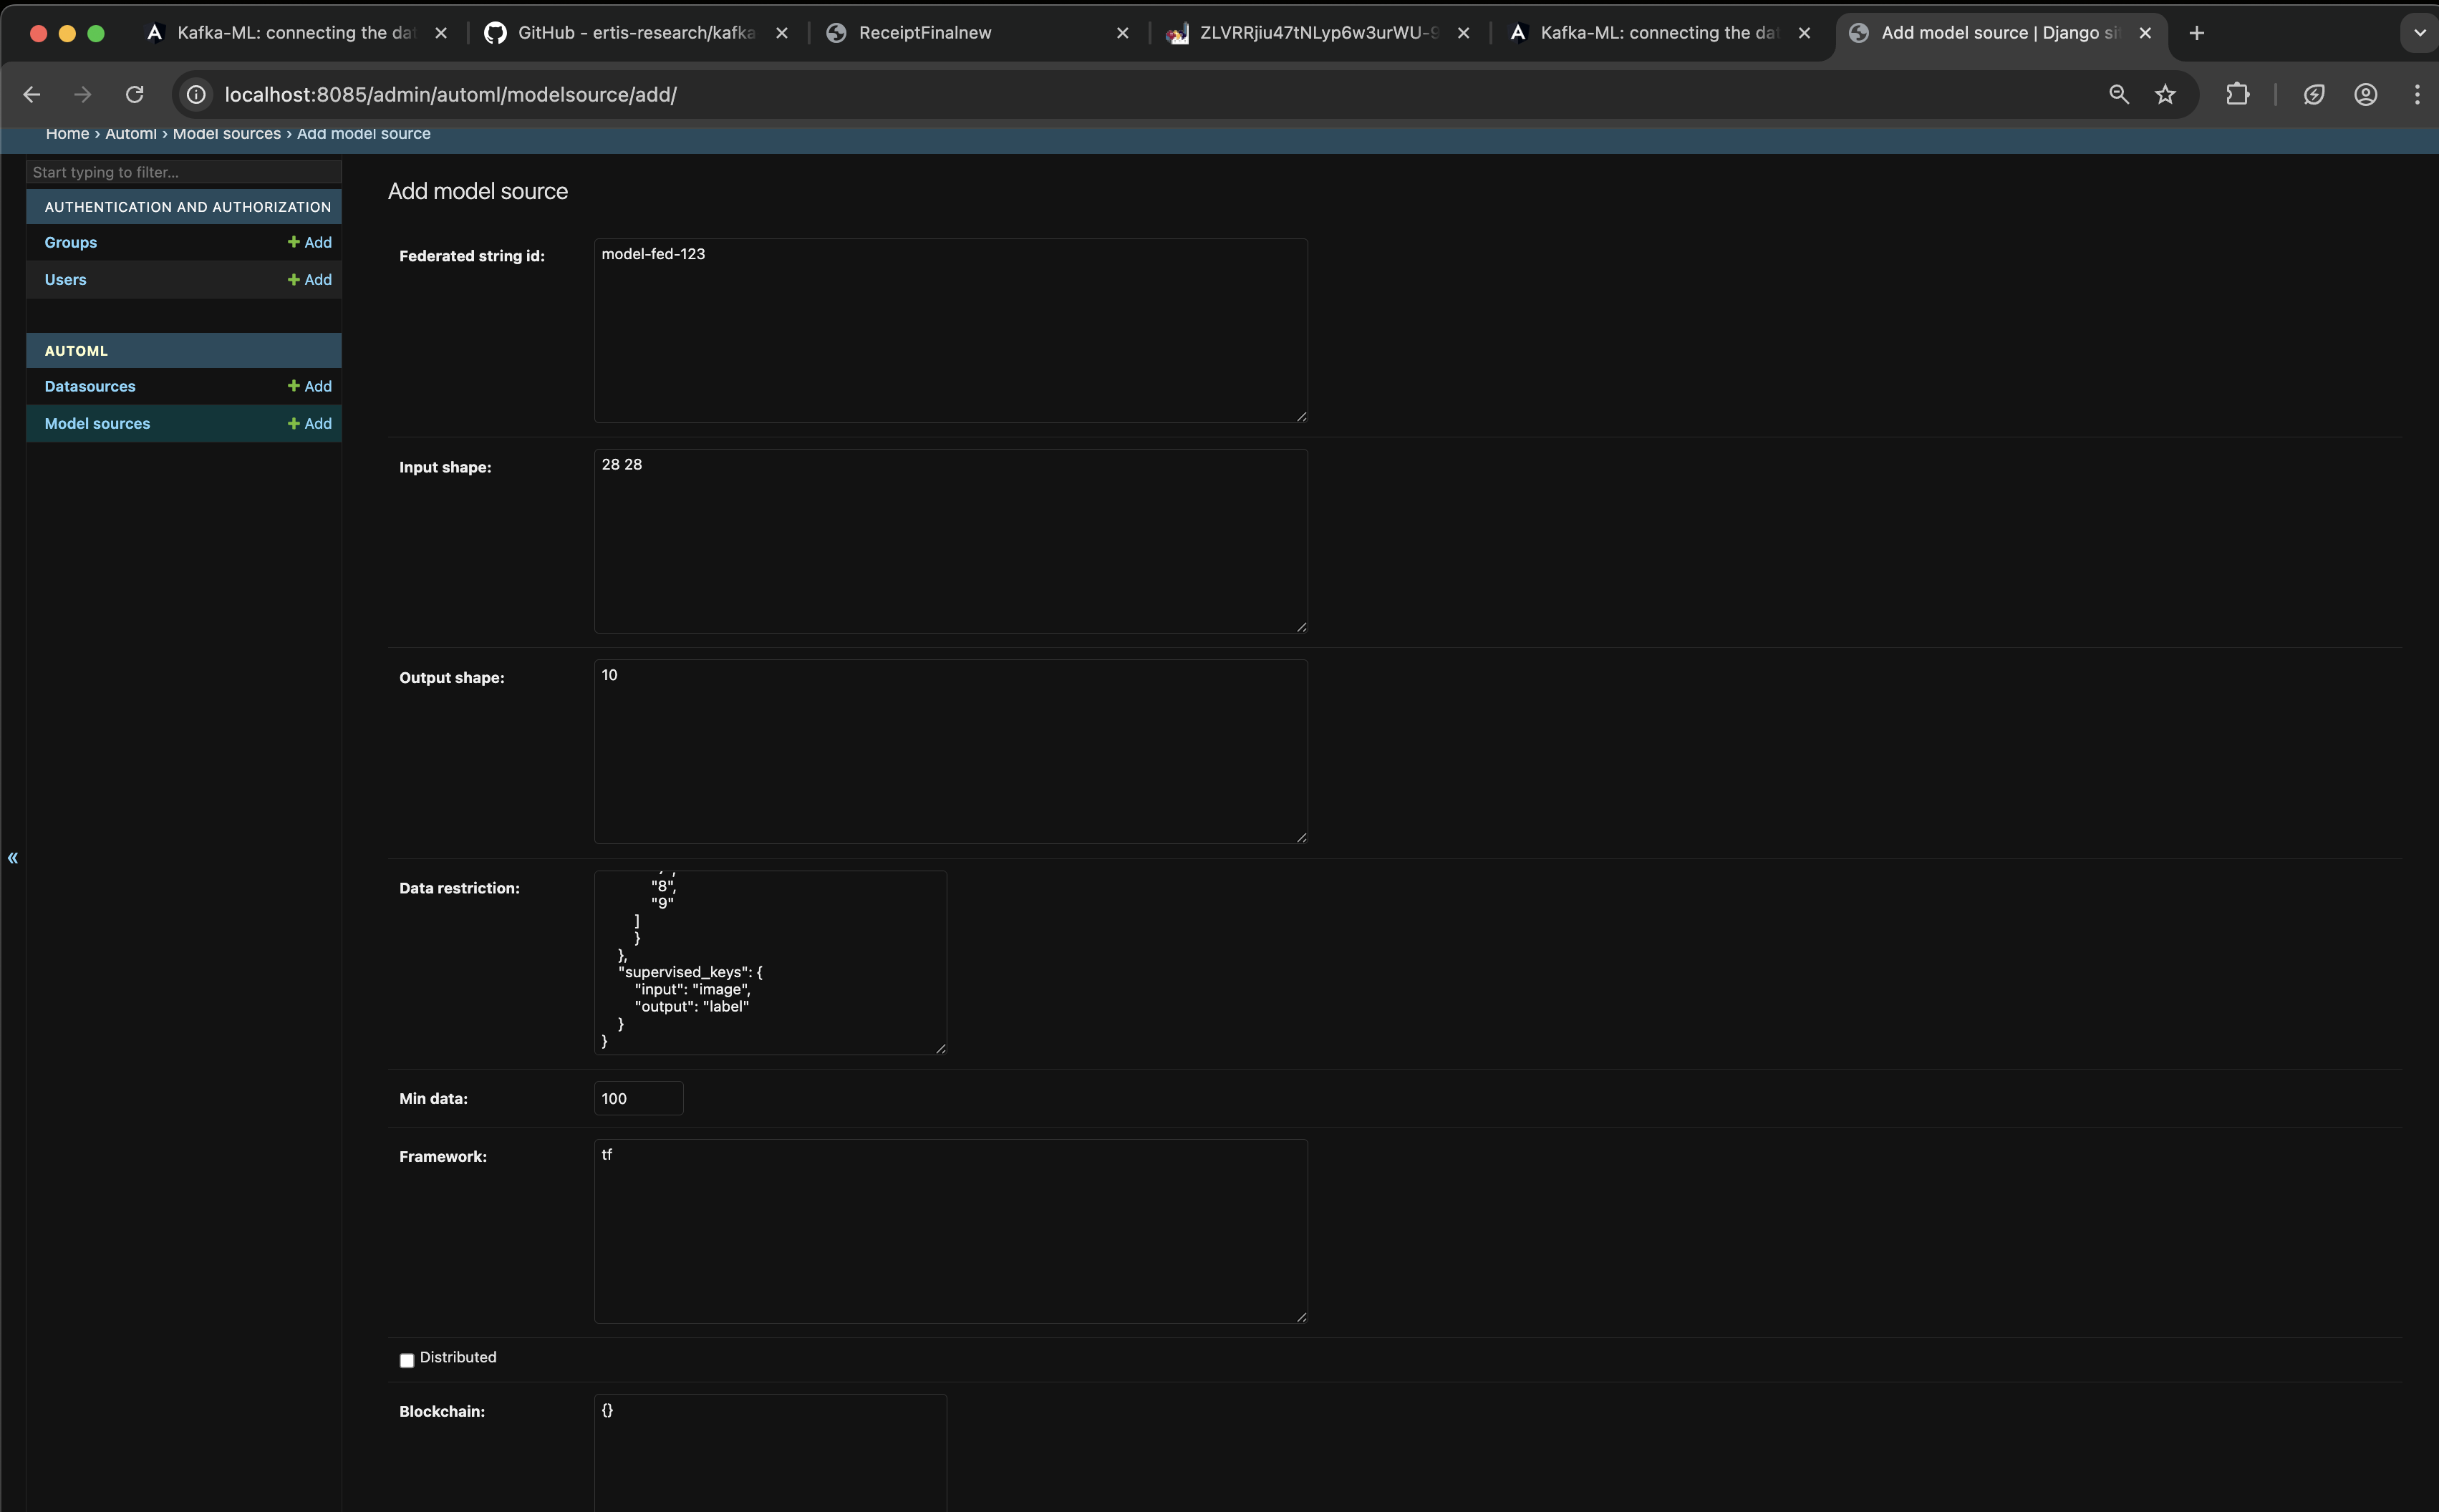
\includegraphics[width=0.7\textwidth]{MWP-Project Report Template - BD-ML-June25/screenshots_federated/6_Model_Control_input.png}
        
        \caption{Submitting the Model Control Input via the Federated Backend.}
        \label{fig:model_control_submission}
    \end{figure}

    \item \textbf{Submission of Data Control Dataset:} Subsequently, the data control dataset was submitted as shown in Fig. \ref{fig:data_control_submission}. For this non-distributed setup, this dataset defines how the available MNIST data should be treated or partitioned for the federated training simulation.
    % Placeholder for a screenshot of submitting data control dataset
    \begin{figure}[h!]
        \centering
         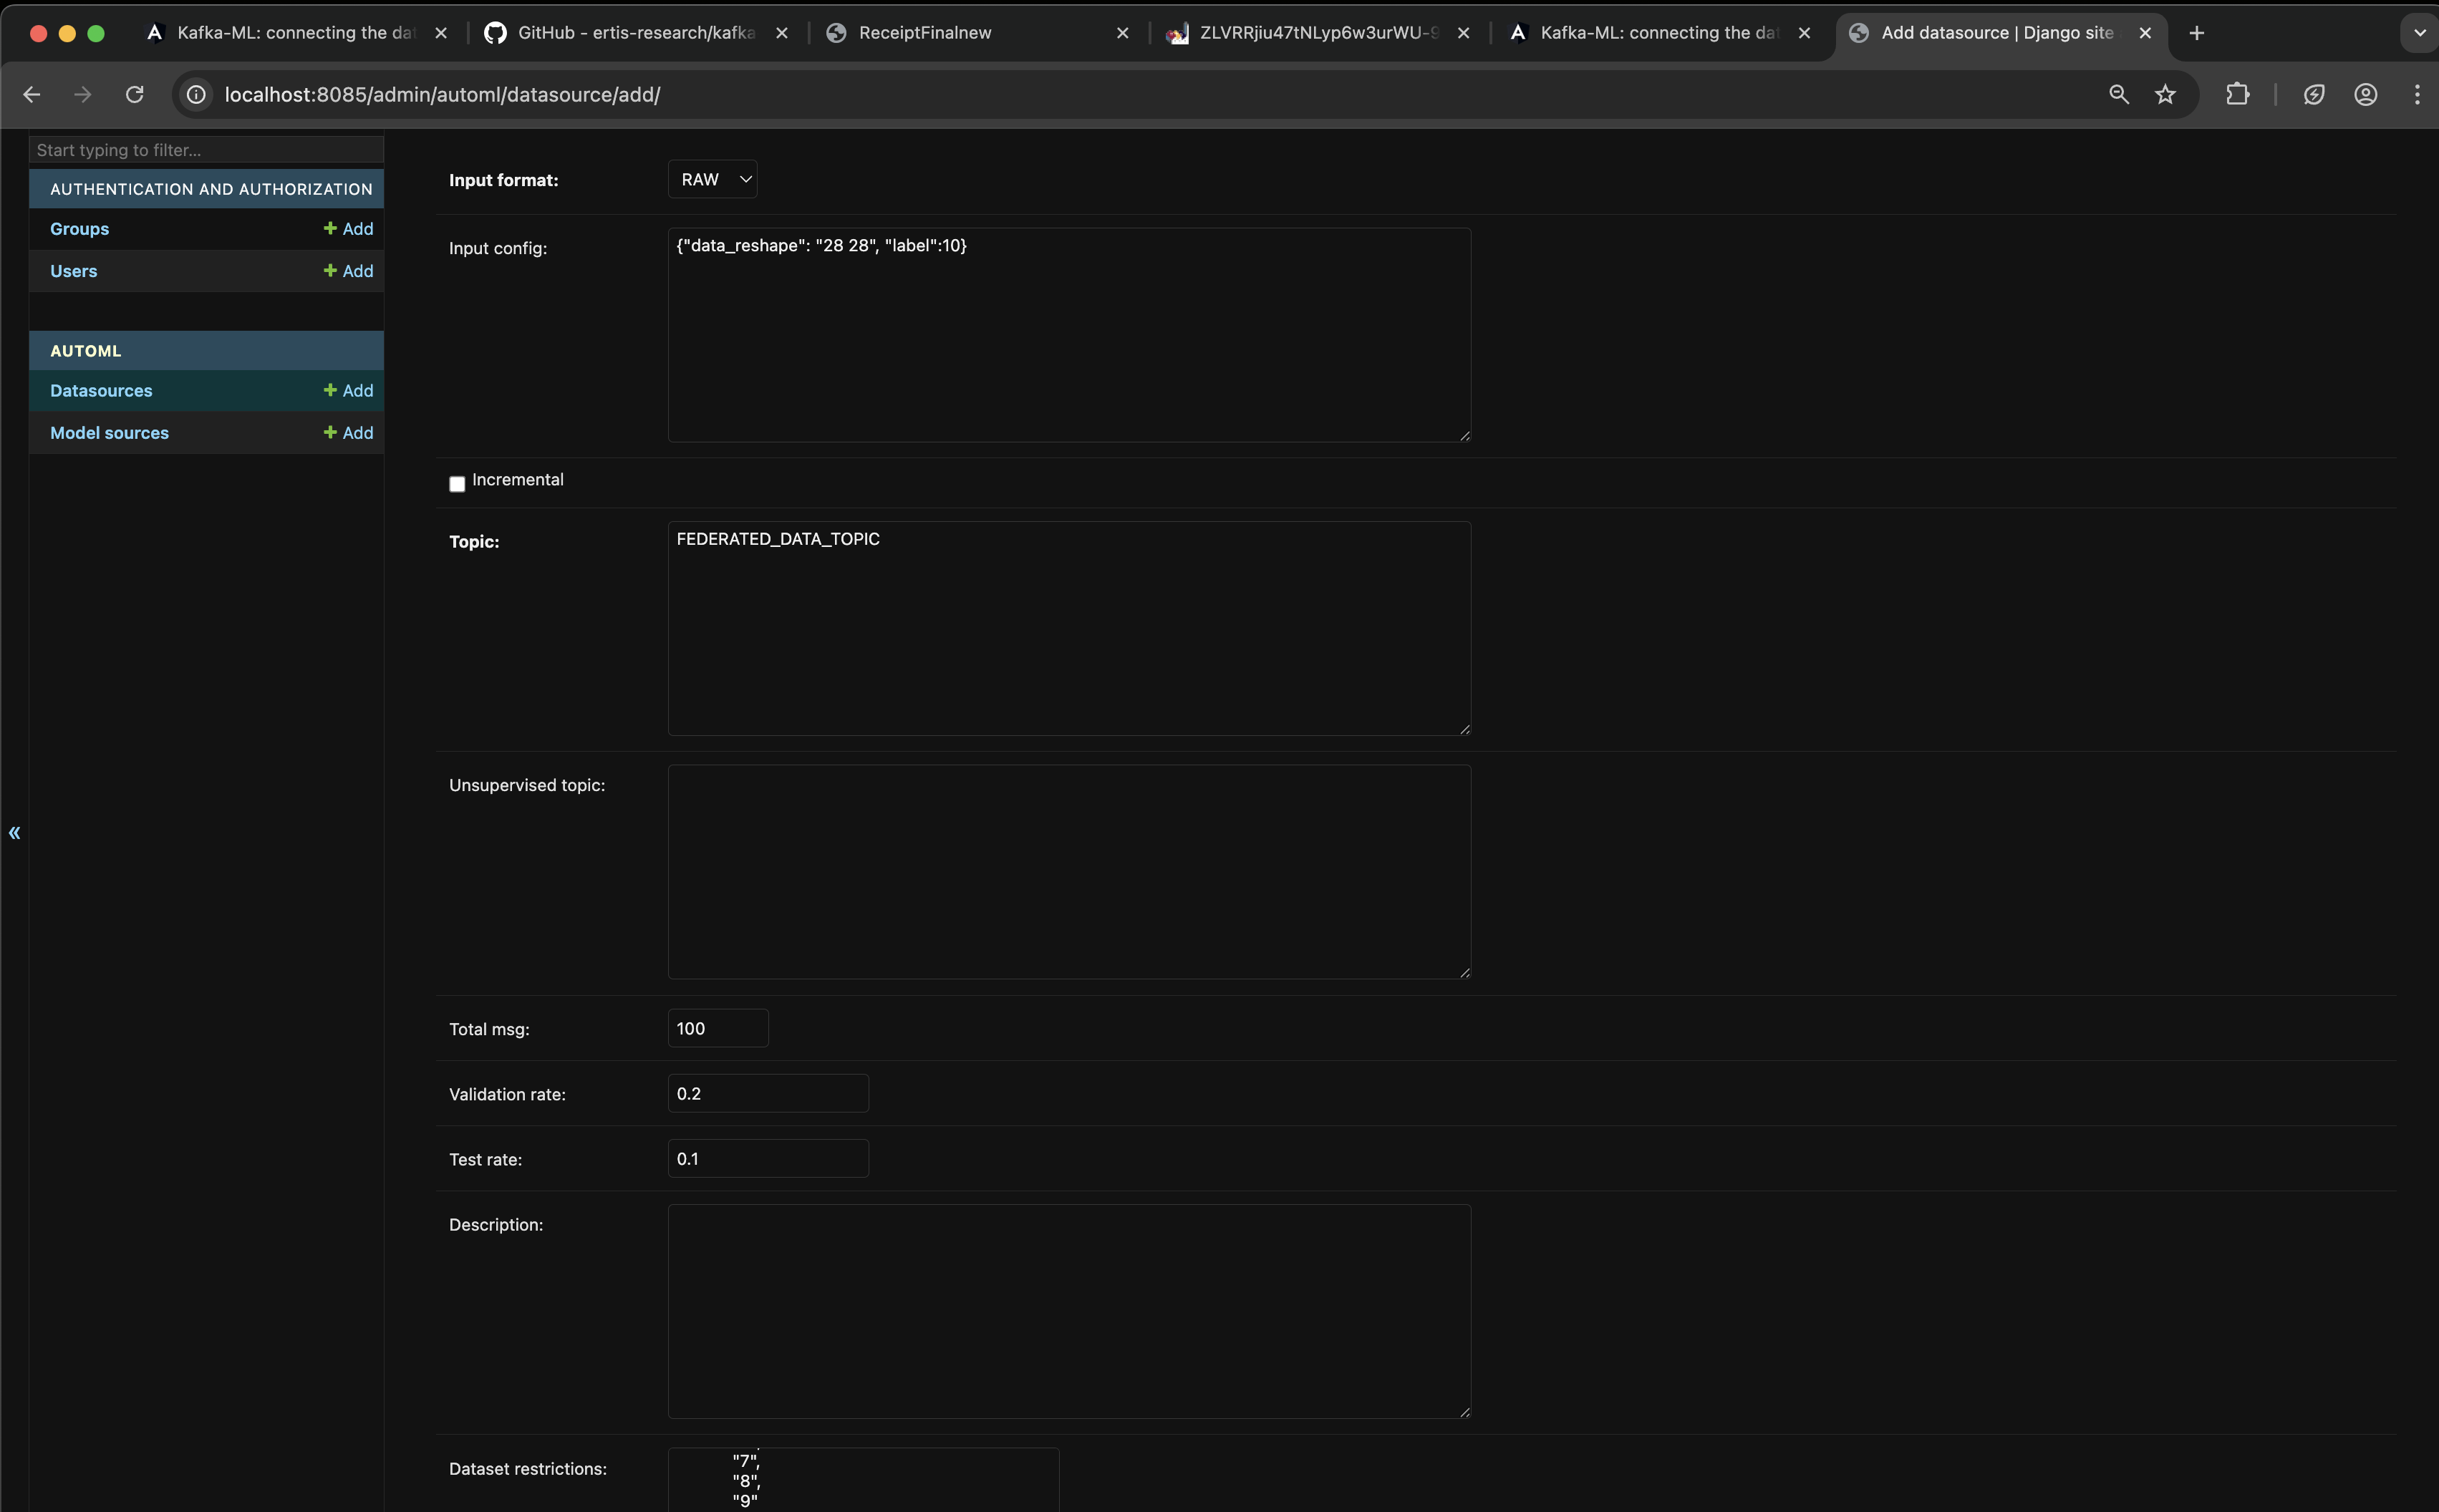
\includegraphics[width=0.7\textwidth]{MWP-Project Report Template - BD-ML-June25/screenshots_federated/5_Data_Control_Input.png}
        \caption{Data Control Submission}
        \label{fig:data_control_submission}
    \end{figure}
\end{enumerate}

\paragraph{Initiating and Observing Federated Training Job}
After the successful submission of both the model control and data control datasets, the federated training job as shown in Fig. \ref{fig:federated_training_job} was initiated. The system then began the process of (simulated) distributed training based on the provided configurations.
% Placeholder for a screenshot of the running training job
\begin{figure}[h!]
    \centering
     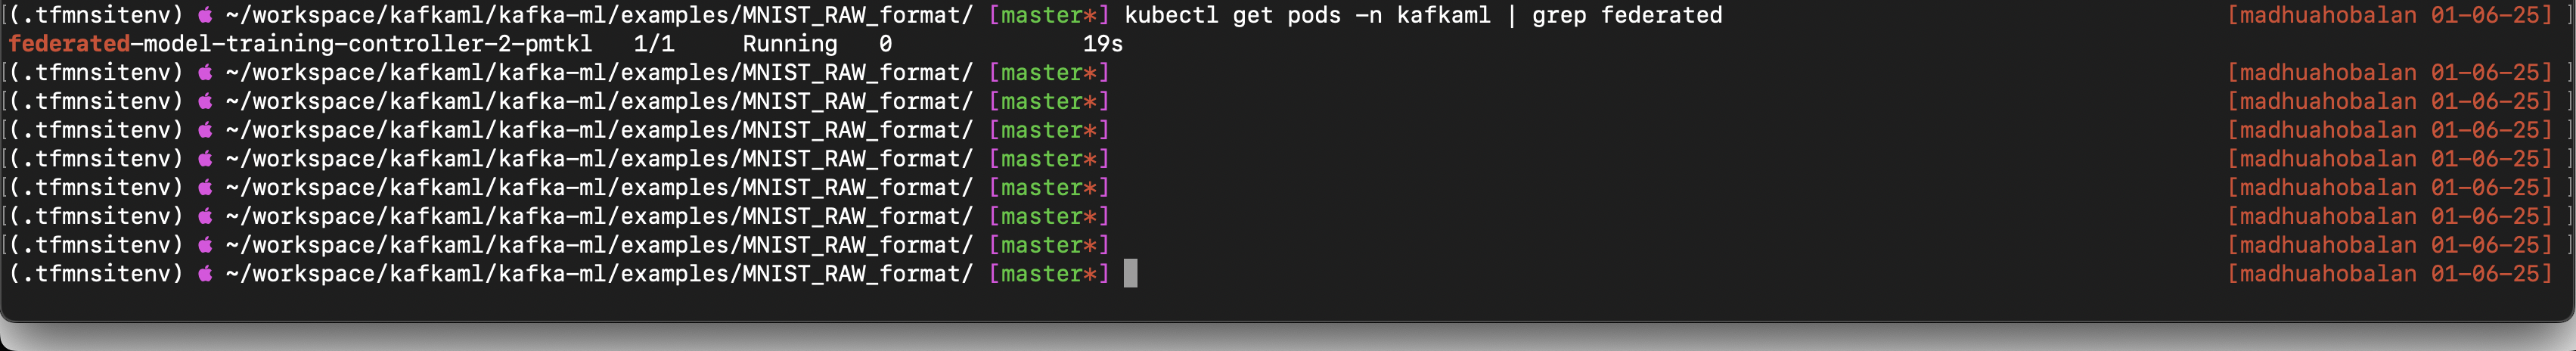
\includegraphics[width=0.8\textwidth]{MWP-Project Report Template - BD-ML-June25/screenshots_federated/7_Federated_Training_Job_Running.png}
   \caption{Federated Training}
    \label{fig:federated_training_job}
\end{figure}

The ability to deploy the federated module and trigger a training job using the control datasets submitted via the Django Admin UI confirmed the operational status of these critical components. This lays the groundwork for expanding to truly distributed data sources and integrating blockchain functionalities as outlined in the project plan.

\subsection{Setup of Single Federated Classic Training for Occupancy Dataset}
\label{subsec:single_fed_classic_occupancy}

With the core federated services validated on MNIST, the next milestone was to exercise the end-to-end pipeline using the room occupancy dataset. This scenario activates the ``single federated classic'' path—one federated worker representing an edge site, but now consuming realistic sensor streams and producing blockchain-ready control records.

\begin{enumerate}
    \item \textbf{Build Kafka-ML base images:} From the repository root, the `./build.sh` script compiled the frontend, backend, model training, model inference, and logger services. Configuration bundles were updated to reference the occupancy-specific Kafka topics.

    \item \textbf{Build federated module images:} Inside `federated-module/`, executing its `./build.sh` produced the federated backend, model/data control loggers, and TensorFlow training worker images, embedding the smart-contract artefacts and wallet credentials required for later auditing.

    \item \textbf{Deploy Kafka-ML core via Kustomize:} Applying `kubectl apply -k kustomize/local` brought up the classic services configured to expose the APIs needed for federated orchestration of the occupancy use case.

    \item \textbf{Deploy federated services via Kustomize:} The command `kubectl apply -k federated-module/kustomize/local` launched the federated backend, control loggers, worker job template, and blockchain helpers. All pods were verified in `Running` state before proceeding.

    \item \textbf{Register model, configuration, and deployment:} Through the Kafka-ML frontend UI a TensorFlow CNN tailored to the occupancy dataset was uploaded, the configuration enabled federated learning, and the deployment bound the model to the occupancy data stream with the desired aggregation cadence.

    \item \textbf{Controller job activation:} Creating the deployment triggered the federated controller job, which fetched the model artefact and control payload from Kafka and acknowledged receipt back to the backend.

    \item \textbf{Backend receives model metadata:} The federated backend stored the architecture and control envelope, persisting hashes to the blockchain where configured, and waited for matching data control messages.

    \item \textbf{Occupancy data ingestion:} A dedicated injector streamed occupancy sensor readings to the Kafka data topic while publishing the control metadata (client ID, shard size, offsets) to the federated data control topic.

    \item \textbf{Collision detection and worker launch:} When matching model and data control entries appeared, the federated backend triggered the single-worker Kubernetes job. The worker retrieved the model weights, consumed the referenced occupancy batch, and commenced local training.

    \item \textbf{Local training and result publication:} After completing its epochs, the worker emitted training and validation metrics, uploaded the updated weights to the aggregation topic, and recorded the contribution on the blockchain. The controller then performed aggregation (trivial with a single worker) and prepared for the next data chunk.
\end{enumerate}

Placeholder panels below will be populated with screenshots from this occupancy walkthrough (build logs, frontend submissions, controller status, worker metrics) once the experiment gallery is finalised.

\begin{figure}[h!]
    \centering
    \begin{adjustbox}{bgcolor=gray!20, padding=0.7em, margin=1ex}
        \begin{tabular}{cc}
            \begin{subfigure}{0.48\textwidth}
                \centering
                \fbox{\parbox{0.9\linewidth}{Placeholder: Kafka-ML build script output}}
                \caption{Kafka-ML Build}
            \end{subfigure} &
            \begin{subfigure}{0.48\textwidth}
                \centering
                \fbox{\parbox{0.9\linewidth}{Placeholder: Federated module build output}}
                \caption{Federated Build}
            \end{subfigure} \\
            \begin{subfigure}{0.48\textwidth}
                \centering
                \fbox{\parbox{0.9\linewidth}{Placeholder: Frontend deployment showing occupancy model}}
                \caption{Frontend Flow}
            \end{subfigure} &
            \begin{subfigure}{0.48\textwidth}
                \centering
                \fbox{\parbox{0.9\linewidth}{Placeholder: Worker training metrics}}
                \caption{Worker Metrics}
            \end{subfigure}
        \end{tabular}
    \end{adjustbox}
    \vskip\baselineskip
    \caption{Placeholder grid for single federated classic occupancy run}
    \label{fig:occupancy_fed_single}
\end{figure}


\subsection{Federated Training with Blockchain Instrumentation}
\label{subsec:fed_blockchain_setup}

The blockchain-enabled run reuses the deployment steps from Section~\ref{subsec:federated_setup_non_distributed}: the same build scripts prepare Kafka-ML and federated images, Kustomize descriptors deploy the pods, and the frontend initiates the model/config/deployment objects. The change lies in the artefacts: controller and worker jobs reference the blockchain-specific manifests, smart-contract credentials, and emit on-chain audit trails during training.

Key behavioural differences from the vanilla run include:

\begin{itemize}
    \item Controller pods carry the `*-blockchain-controller` naming convention and, after each round, log transaction hashes confirming that model control messages were notarised on the contract.
    \item Federated workers publish their contribution metadata to the blockchain, producing log entries that show token reward calculations (loss/accuracy deltas) before pushing aggregation control messages.
    \item The backend wallet ledger reflects credit transfers per round, enabling traceable incentive payouts per client.
\end{itemize}

Placeholder screenshots below will be populated with the blockchain-specific controller and worker logs, contract dashboards, and reward summaries once the full experiment set is captured.

\begin{figure}[h!]
    \centering
    \begin{adjustbox}{bgcolor=gray!20, padding=0.7em, margin=1ex}
        \begin{tabular}{cc}
            \begin{subfigure}{0.48\textwidth}
                \centering
                \fbox{\parbox{0.9\linewidth}{Placeholder: Blockchain-enabled controller pod logs}}
                \caption{Controller Logs}
            \end{subfigure} &
            \begin{subfigure}{0.48\textwidth}
                \centering
                \fbox{\parbox{0.9\linewidth}{Placeholder: Worker reward calculation output}}
                \caption{Reward Metrics}
            \end{subfigure} \\
            \begin{subfigure}{0.48\textwidth}
                \centering
                \fbox{\parbox{0.9\linewidth}{Placeholder: Smart contract dashboard snapshot}}
                \caption{Contract Dashboard}
            \end{subfigure} &
            \begin{subfigure}{0.48\textwidth}
                \centering
                \fbox{\parbox{0.9\linewidth}{Placeholder: Backend wallet transaction list}}
                \caption{Wallet Activity}
            \end{subfigure}
        \end{tabular}
    \end{adjustbox}
    \vskip\baselineskip
    \caption{Placeholder grid for blockchain-instrumented federated training}
    \label{fig:blockchain_fed_placeholders}
\end{figure}


